\documentclass{scrreprt}

\usepackage{rotating}
\usepackage{amsmath,amssymb}
\usepackage[utf8]{inputenc}
\usepackage{xcolor}
\usepackage[top=30mm]{geometry}
\usepackage{graphicx}
\usepackage{hyperref}
\usepackage{fancyhdr}
\pagestyle{fancy}

\fancyhf{}
\addtolength{\headheight}{0.0cm}  
\cfoot{\thepage}
\fancypagestyle{plain}{\pagestyle{fancy}}

\usepackage[backend=biber,natbib,style=apa]{biblatex}
\addbibresource{references.bib}

\setlength{\parindent}{0pt}
\setlength{\parskip}{10pt}

\author{First Name LAST NAME}
\date{\today}

\begin{document}
\begin{titlepage}

\begin{figure}
\begin{minipage}{0.50\columnwidth}
\begin{flushleft}

\includegraphics[width=3cm]{logos/ethz.jpg}
\end{flushleft}
\end{minipage}
\begin{minipage}{0.50\columnwidth}
\begin{flushright}

\includegraphics[width=3cm]{logos/sdsc.jpg}
\end{flushright}
\end{minipage}%
\end{figure}%

\vspace*{5cm}
\newcommand{\HRule}{\rule{\linewidth}{0.5mm}}
\newcommand{\hRule}{\rule{\linewidth}{0.25mm}}

\center
\rule{\linewidth}{0.25mm}\\[0.4cm]
{\vspace{0.2in}\Huge \sffamily \bfseries Seismic Phase Association }\\~~\\
\rule{\linewidth}{0.5mm}\\[2.5cm]
{\scshape \large Machine Learning Phase Association for Underground Laboratory Acoustic Emission Data}\\~~\\
\vspace*{5cm}
\begin{minipage}{0.45\textwidth}
\begin{flushleft} \large
\emph{Author:}\\
Nicolas \textsc{Schmid} 
\end{flushleft}
\end{minipage}
\begin{minipage}{0.45\textwidth}
\begin{flushright} \large
\emph{Supervisors:} \\
Dr. Simon \textsc{Dirmeier} \\
Dr. Men-Andrin \textsc{Meier} \\
Prof. Dr. Fernando \textsc{Perez-Cruz}
\end{flushright}
\end{minipage}\\[1cm]
{\large \today}
\end{titlepage}

\begin{abstract}
\begin{center}
{\LARGE \sffamily\bfseries Abstract}
\end{center}
This work addresses the challenge of phase association in seismic monitoring under conditions of high event rates and small magnitudes, such as those found at the BedrettoLab Underground Laboratory. Traditional phase association methods often fall short in such complex scenarios due to their inability to handle rapid sequences of seismic events correctly. The effectiveness of various algorithms, including the GaMMA method based on Bayesian Gaussian mixture models and PyOcto, which uses a structured octotree approach, were compared. We generated synthetic datasets reflecting realistic seismic activity to assess performance. Our findings indicate, that while both methods perform well at lower event rates, GaMMA provides superior performance as event rates increase, particularly when configured with refined parameters and adapted to use modified ground motion prediction equations. Moreover, this report proposes modifications to improve these algorithms' applicability to real-world seismic monitoring at geothermal sites and similar settings. 
\end{abstract}

\chapter{Introduction}
\section{Earthquake Monitoring}
\subsection{Detection and Localization}
Earthquakes are recorded by a network of seismometers distributed across various locations. The location and magnitude of a single event can be determined by analyzing the maximum amplitudes and arrival times of seismic waves at different stations.

Earthquakes generate two primary types of seismic waves: the faster P-waves and the slower S-waves. By knowing the propagation speed of these waves, the difference in their arrival times at a station can be used to calculate the distance to the event. Therefore, with recordings of the P- and S-wave arrival times at multiple stations, the origin of the earthquake can be accurately located. While the simplest models assume a constant wave speed, more complex and realistic models are also available.

\begin{figure}[ht]
    \centering
    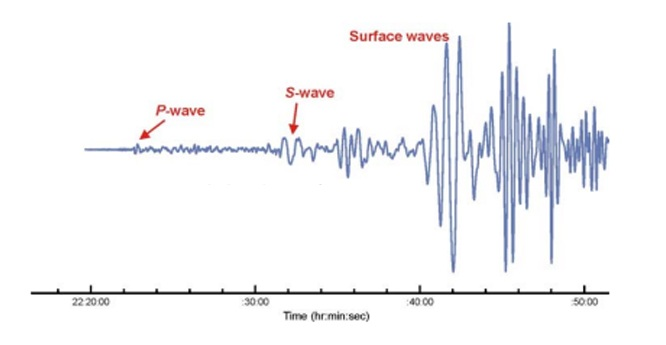
\includegraphics[width=0.5\linewidth]{plots/Wave_arrival_BGS.jpg}
    \caption{P- and S-wave arrivals on a seismogram.\citep{fig-waves}}
    \label{fig:wave_arrivals}
\end{figure}

Similarly, by using the recorded amplitude of ground motions at a station and the distance to the event, the magnitude can be calculated. There are multiple models available for this calculation, as well as several different magnitude scales.

Many of the steps involved in the procedure of earthquake detection and localization have traditionally been performed manually and still require manual intervention. However, Machine Learning algorithms are being developed to improve and automate this process.

\subsection{Phase Association}
Phase association refers to the challenge of determining which wave arrivals at different stations, also known as "picks," were caused by the same earthquake. Accurately solving this problem is essential for determining the earthquake's location and magnitude. The problem is trivial as long as the time interval between two earthquakes is longer than the S-wave travel time from the hypocenter to the furthest station (Fig. \ref{fig:arrival}, left). However, when events occur in quick succession, the separation of picks becomes increasingly complex (Fig. \ref{fig:arrival}, right).

\begin{figure}[ht]
    \centering
    \begin{minipage}{0.49\textwidth}
        \centering
        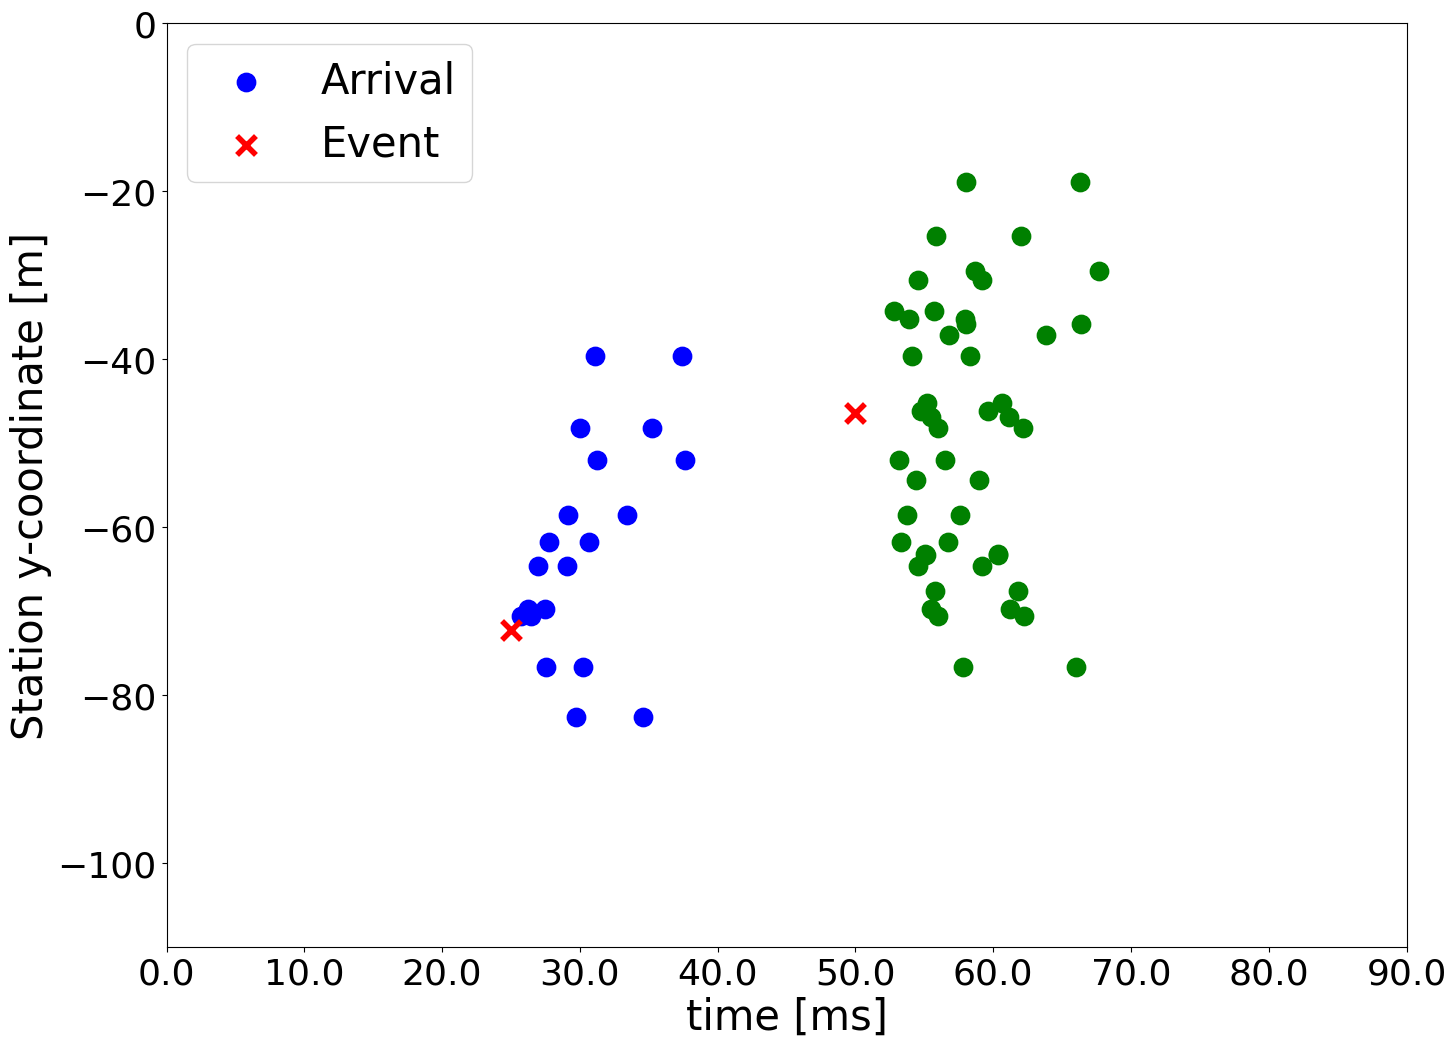
\includegraphics[width=\textwidth]{plots/separated.png}
    \end{minipage}
    \hfill
    \begin{minipage}{0.49\textwidth}
        \centering
        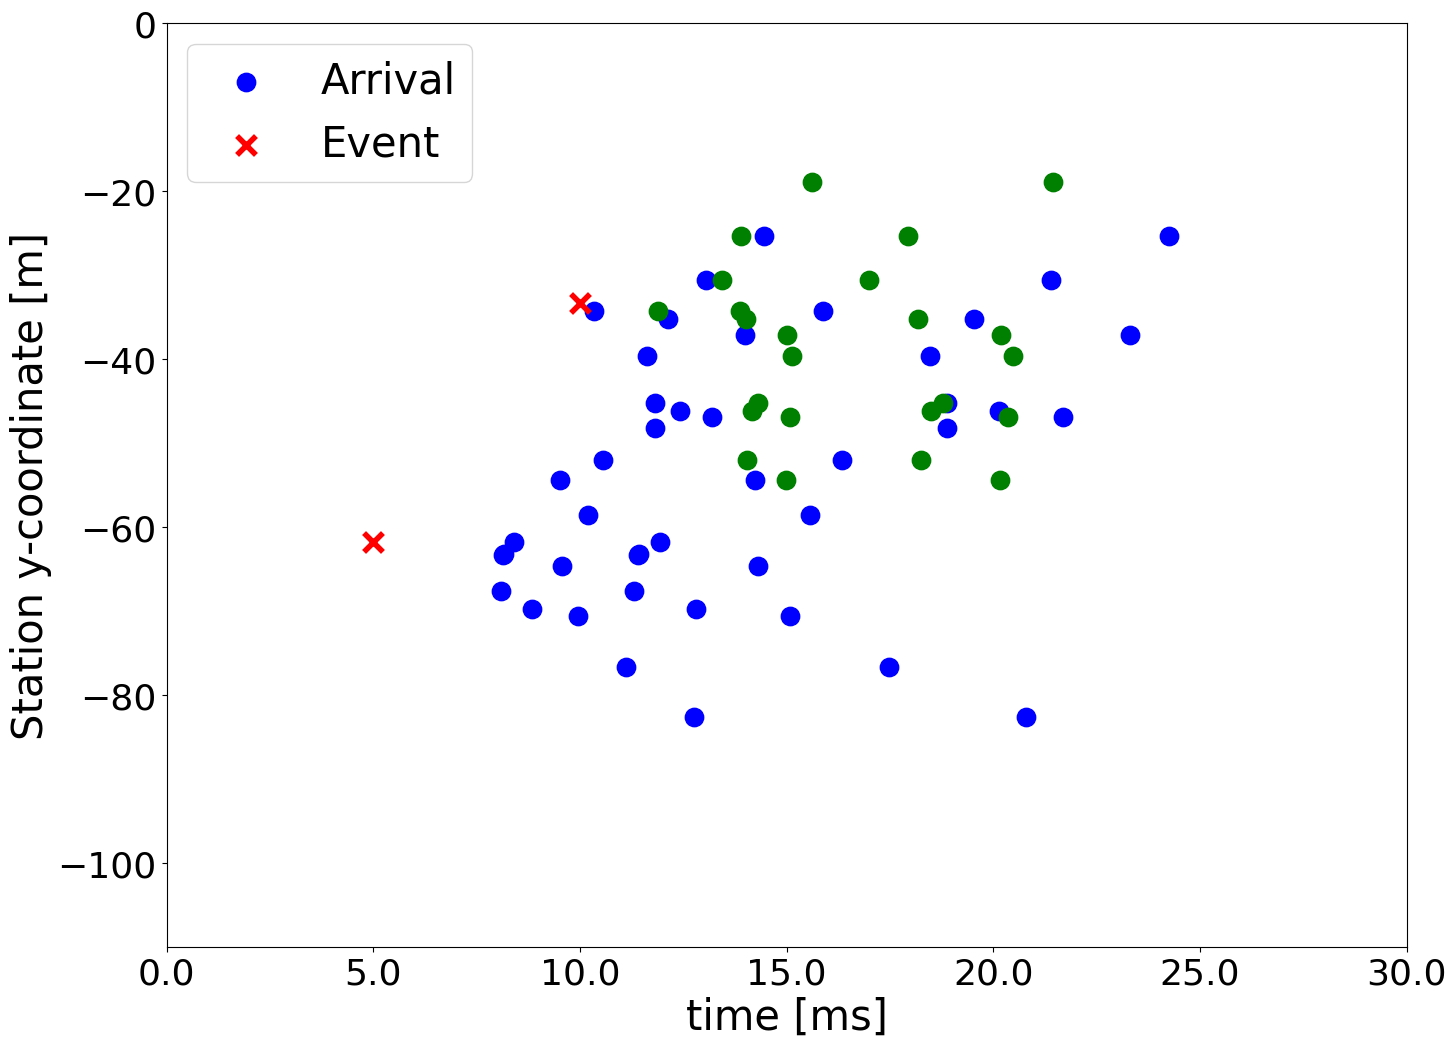
\includegraphics[width=\textwidth]{plots/unseparated.png}

    \end{minipage}
    \caption{\label{fig:arrival}Arrivals of seismic waves of 2 events at multiple stations.}
\end{figure}

\section{Motivation}

Country-wide earthquake monitoring networks typically record a relatively small number of earthquakes on a normal day and phase association is not an issue. However, during a large event, a significant increase in the number of small earthquakes is expected. It has been observed \citep{amatrice}, that in such cases, many small events that would normally be detected, may be missed, to a large degree because the phase association is not solved correctly anymore.

The BedrettoLab Underground Laboratory conducts research in the fields of geothermal energy and earthquake physics. A large array of both classical and novel sensor technologies has been deployed to monitor geophysical processes. Seismic waves can be recorded with high precision using acoustic emission sensors and earthquakes down to magnitudes as low as -4 and -5 are being detected. As we detect smaller earthquakes, the number of detected events increases exponentially due to the inverse relationship between magnitude and rate, making phase association a critical bottleneck in various applications.

The objective of this work is to identify and refine a method for phase association suitable for this scale of operation. Performance assessments and practical applications of existing methods have largely been limited to regional or national scales. Thus, any chosen method may require modifications, comprehensive testing, and careful configuration to function effectively under these conditions. Optimally, recommendations and insights for future developments in this field can be provided.

\chapter{Background}

Various methods have been developed to address the problem of phase association. Traditionally, these methods rely on back-projection, where space and time are partitioned to search for a possible origin of a set of picks. In recent years, numerous machine learning methods, ranging from deep learning to statistical techniques, have been proposed.

\section{Previous Work}

A well-tested approach is REAL \citep{real}, where an algorithm associates picks to each other within a specific time window, and then, only in a second step, attempts to match travel times to a potential location.

Other methods leverage deep learning techniques. \citet{pairwise} use convolutional neural networks to analyze waveforms of arrivals and classify them pairwise, determining if they belong to the same event. Similarly, PhaseLink \citep{phaselink} utilizes Recurrent Neural Networks to address the association problem. It selects a root pick together with a sequence of consecutive picks, predicting whether each of those picks belongs to the root pick.

In GENIE, \citet{gnn} implemented a complex Graph Neural Network that learns the spatial and temporal structure of the seismic network and its source region, predicting associations as well as locations of earthquakes. Another approach using GNNs is proposed by \citet{plan4} in their PLAN4 algorithm, which integrates picking, associating, and locating earthquakes in a single approach.

\subsection{Method Selection}
The primary criterion for method selection in this case is the ability to associate events in an area at least 100 times smaller than typically tested, and to handle earthquake rates 100 to 1000 times higher. Moreover, the chosen method should be capable of processing picks detected by an existing deep learning phase picker. It does not however, need to provide reliable earthquake locations or magnitude estimations, as robust methods for these tasks already exist based on the associated phase detections.

After reviewing the aforementioned algorithms and conducting preliminary tests on several of them, the GaMMA approach \citep{gamma} was selected. This method, based on Bayesian Gaussian mixture model clustering \citep{bishop}, has shown promising performance. It is intuitive, physics-informed, extensible \citep{neuma}, and tested in the field \citep{quakeflow}. The method will be described in more detail in the subsequent chapter.

For reference, and to assess whether the traditional back-projection approach could be applicable to this specific problem, PyOcto \citep{pyocto} was chosen. This associator optimizes the ability to process large volumes of picks, such as those produced by deep learning phase pickers, using an optimized data structure inspired by an octotree. It divides the space and time domain into 4D volumes called nodes. Nodes containing possible earthquake origins are retained and subdivided into smaller volumes, while nodes unlikely to contain an event origin are discarded.

\chapter{Method}

\section{Data}
The definition of the phase association problem from the dataset perspective is straightforward. The information available for phase association includes the locations of seismic stations, along with the arrival times, phase types, and amplitudes of the recorded seismic waves. Inversely, given the location, time, and magnitude of an event, we can easily compute the theoretical arrival time and amplitude at each station. Therefore, for the scope of this work, exclusively synthetic data was used, primarily because the ground truth is known, allowing for a comprehensive assessment of the performance of various methods.

As a first step, catalogues of earthquakes, including magnitude, time, and location are created. For the magnitudes, we utilized the well-known \citet{GR1944} relationship and magnitudes were drawn from an exponential distribution. To generate the timestamps of the events, we use a Poisson process with rate parameter $r$ to generate intervals between arrivals, meaning that over a prolonged period we expect a constant rate of events.

\begin{figure}[ht]
    \centering
    \begin{minipage}{0.49\textwidth}
        \centering
        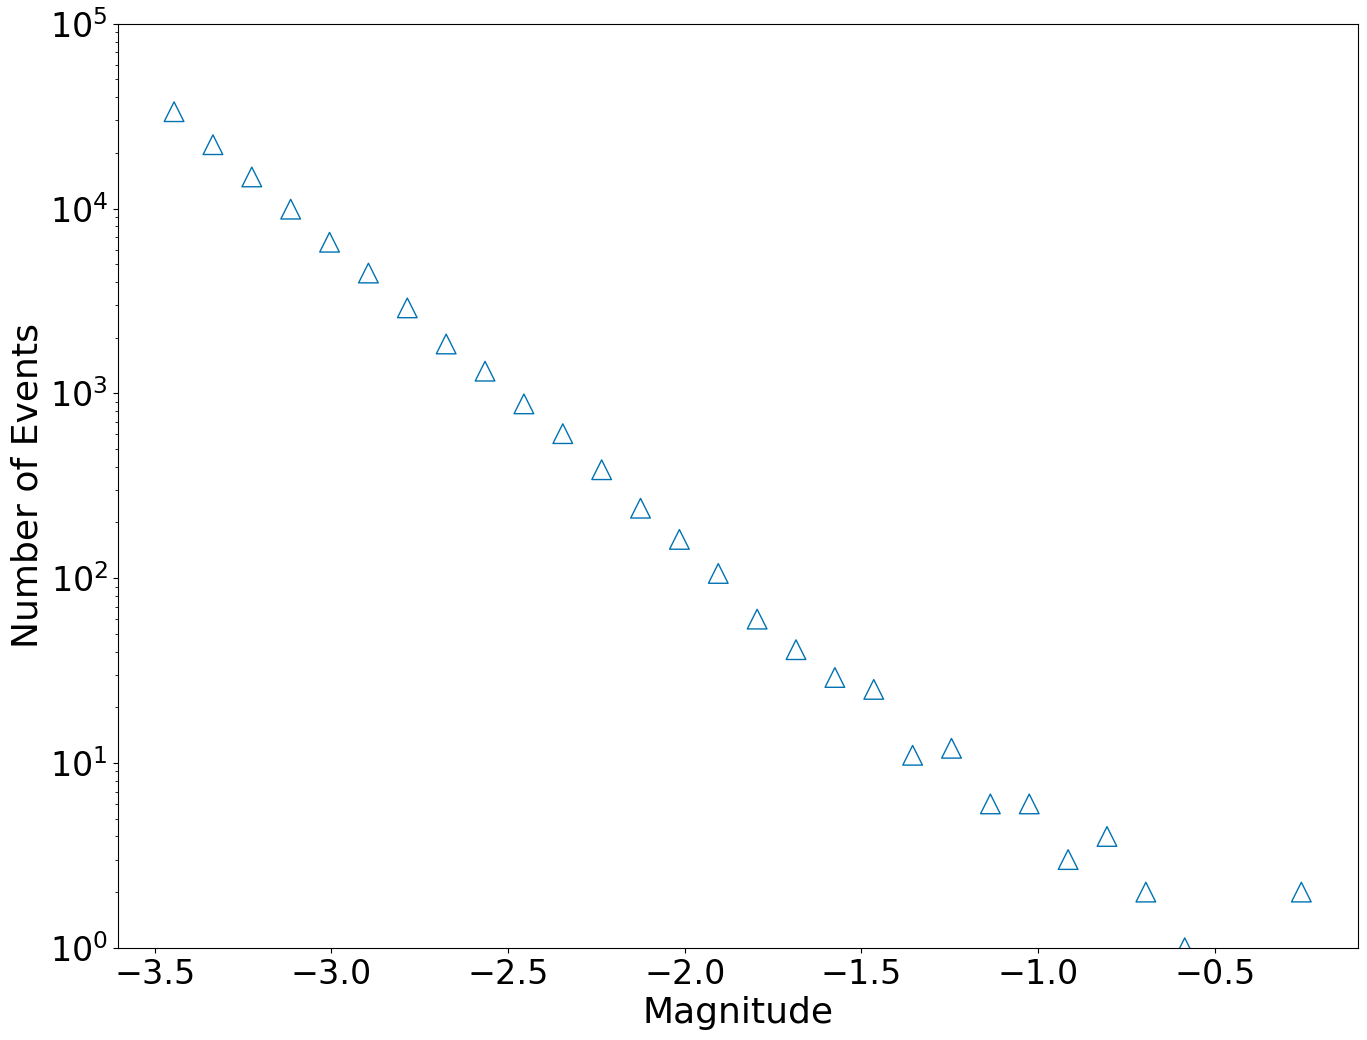
\includegraphics[width=\textwidth]{plots/fmd.png}
    \end{minipage}
    \hfill
    \begin{minipage}{0.49\textwidth}
        \centering
        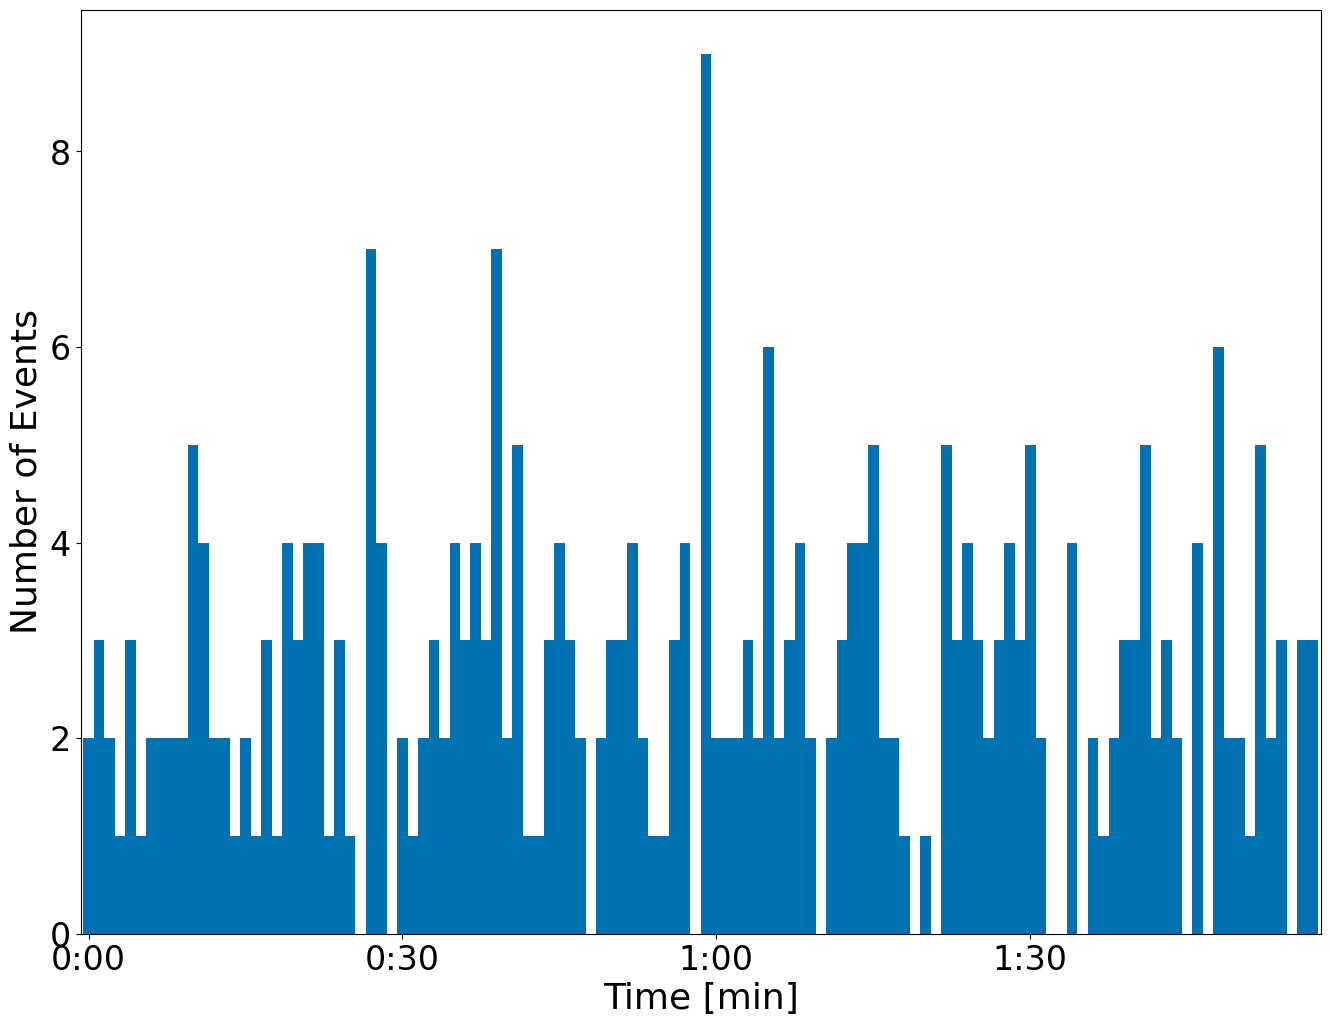
\includegraphics[width=\textwidth]{plots/rates.png}

    \end{minipage}
    \caption{\label{fig:cat}On the left: Frequency-magnitude distribution of 100'000 generated events. On the right: Event rates per second over 2 minutes, with $r=2.5$.}
\end{figure}

The spatial distribution of events was generated using a physics-based workflow, which samples event locations based on a focal mechanism, magnitude, and stress drop of a main event. A finite source around the hypocentre is computed as per \citet{Meier2014}. Subsequently, the resulting crack radius is used to calculate a stress profile according to \citet{Dietrich94}. Aftershocks are then sampled as a function of distance from the hypocentre based on this stress profile. The locations of the seismic stations and the general area of the events were chosen to match the real locations of sensors available at BedrettoLab.

\begin{figure}[ht]
\centering
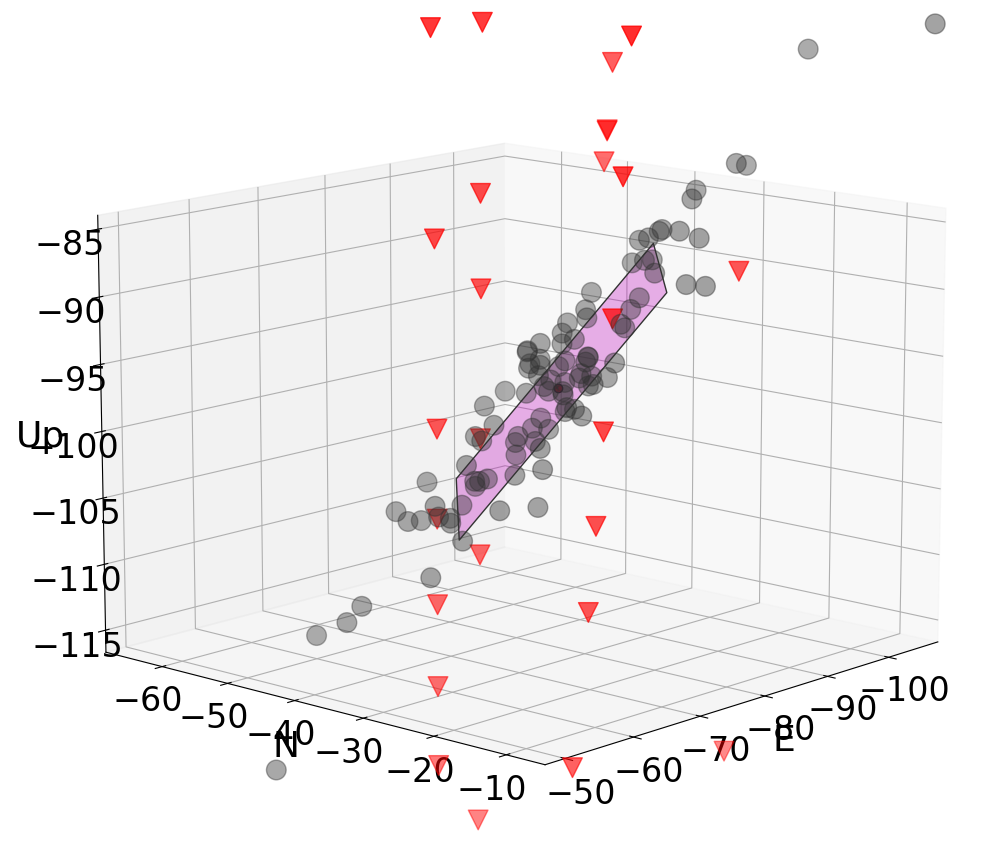
\includegraphics[width=0.65\linewidth]{plots/events_3d.png}
\caption{\label{fig:3d}Distribution of events (black) and stations (red) in space, together with the slip patch plane.}
\end{figure}

The arrival times of the P- and S- waves of each event at every station is then calculated using a uniform velocity model which assumes constant wave travel velocities $v_p$ and $v_s$ from the hypocentre to the station location. 
\begin{equation} \label{vel}
    \begin{aligned}
    t_{ik} & = \frac{d_{ik}}{v} + t_k \\
    \tilde{t}_j & = t_{ik} + \varepsilon
    \end{aligned}
\end{equation}
where $\tilde{t_j}$ is the arrival time of pick $j$ (at station $i$), $t_{ik}$ is the theoretical arrival time of a wave from event $k$ at station $i$, $d_{ik}$ is the distance between event $k$ and station $i$ in meters, $v$ is the wave travel speed in m/s, $t_k$ is the origin time of event $k$ and $\varepsilon$ is a noise term \(\varepsilon \sim \mathcal{N}(0, \nu \cdot \frac{d_{ik}}{v})\) with $\nu$ controlling the amount of noise of the travel times.


\begin{figure}[ht]
    \centering
    \begin{minipage}{0.49\textwidth}
        \centering
        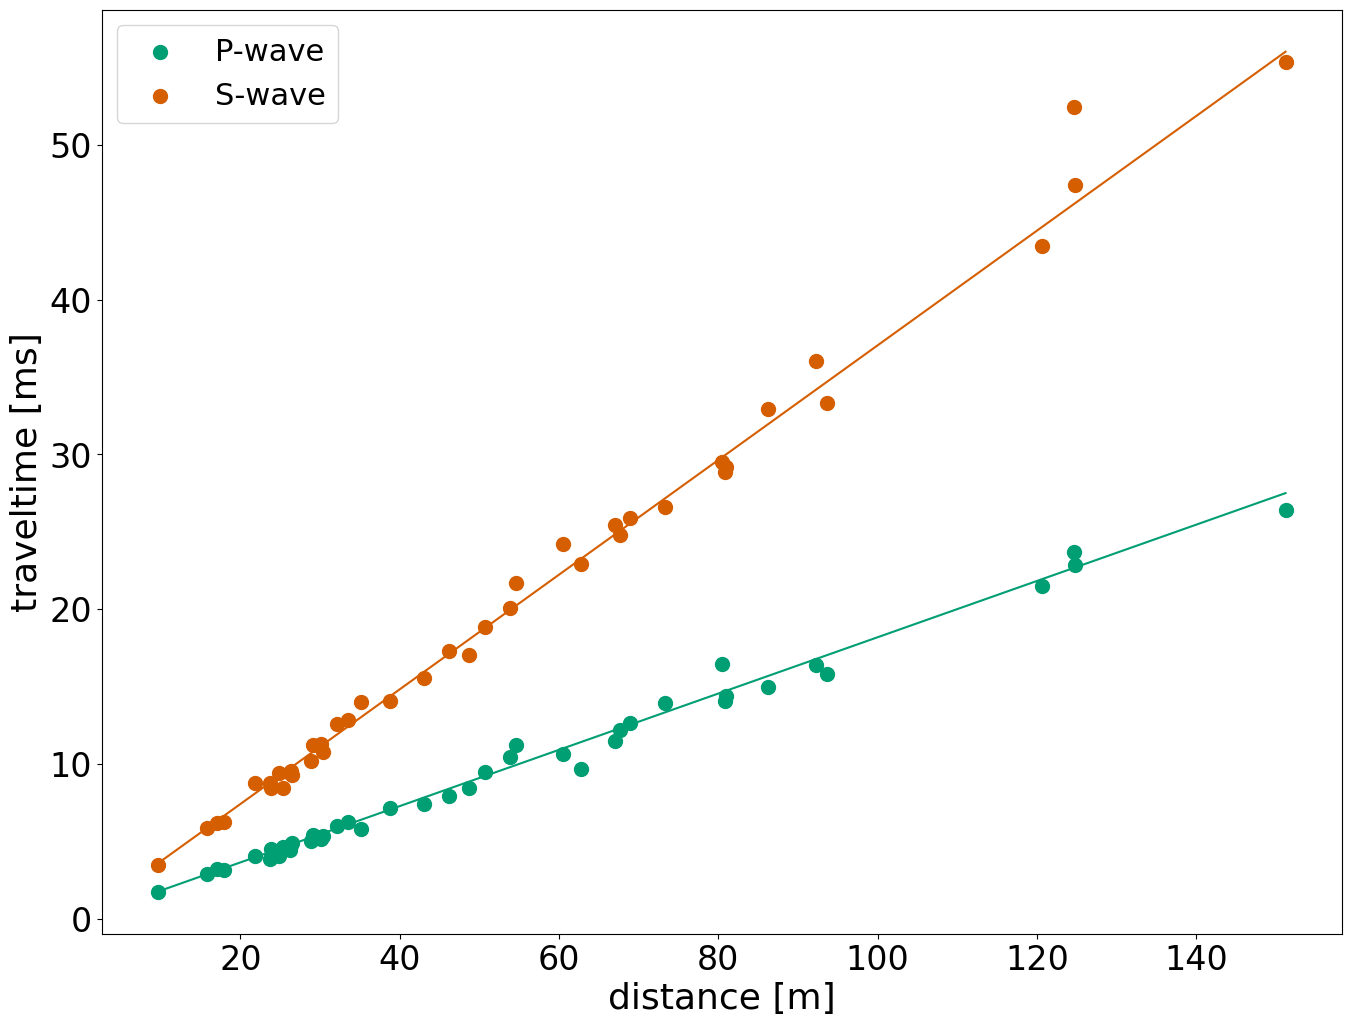
\includegraphics[width=\textwidth]{plots/noise_traveltime.png}
    \end{minipage}
    \hfill
    \begin{minipage}{0.49\textwidth}
        \centering
        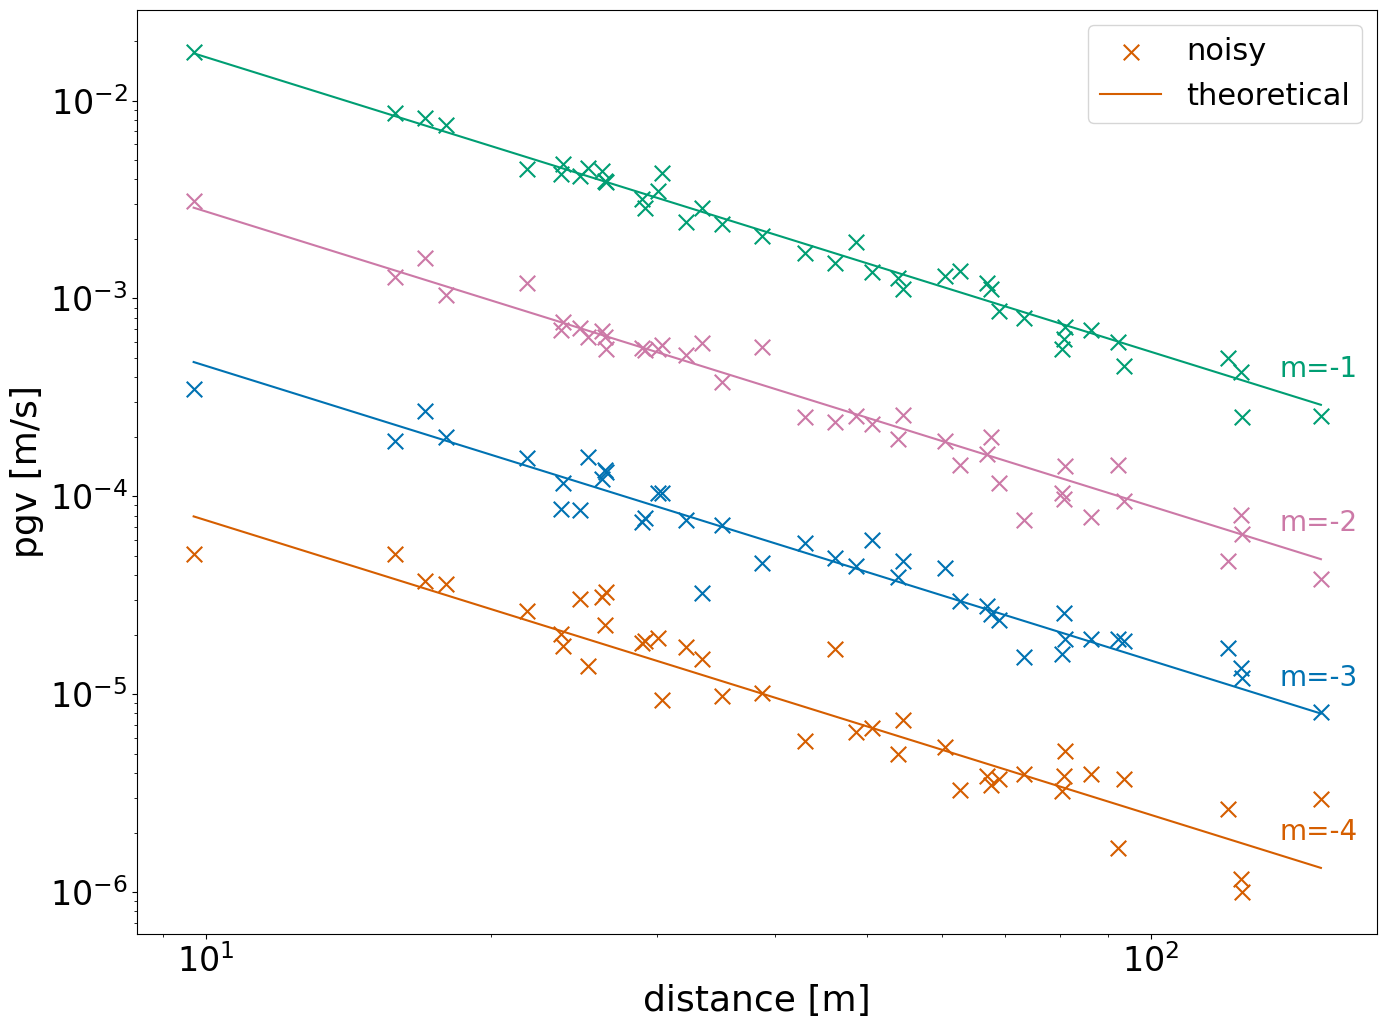
\includegraphics[width=\textwidth]{plots/noise_amplitude.png}

    \end{minipage}
    \caption{\label{fig:noise}Theoretical vs noisy values at the stations as a function of distance to the hypocentre. Left: travel time vs distance with $\nu=0.05$, right: amplitude vs distance with $\tau=0.025$. }
\end{figure}

The amplitude of the wave recorded at each station is calculated using a ground motion prediction equation (GMPE) by \citet{butler1993apquant} based on distance and magnitude.

\begin{equation}\label{eq:gmpe}
    \begin{aligned}
    log_{10}a_{ik} & = 0.343+0.775m - 1.423\log_{10}(d_{ik}) \\
    log_{10}\tilde{a}_j & = log_{10}a_{ik} + \varepsilon
    \end{aligned}
\end{equation}

Where $m$ is the magnitude, $\tilde{a}_j$ is the measured amplitude of pick $j$ at station $i$, $a_{ik}$ is the theoretical amplitude at station $i$ triggered by event k, and $\varepsilon \sim \mathcal{N}(0, \tau\cdot|log_{10}a_i|)$ with $\tau$ controlling the amount of noise in the amplitude.

As measurements are noisy and false positives happen frequently, we added false picks to the data. The amount of false picks was assumed at around 10\%, recorded at randomly sampled stations and times, with amplitudes sampled from the true set and some added noise. 

\section{Performance Calculation}

Many phase association algorithms, including PyOcto and GaMMA, provide a preliminary event location and time for the detected pick clusters. However, these algorithms explicitly state that the initial location is merely a first estimate and should be recalculated using a dedicated method. Therefore, we evaluate the performance of these algorithms based on the clustering of the picks.

The general problem definition is such that all picks from the same event should form a cluster. Those clusters are labeled with integers from $0$ to $k$, with noise picks assigned the label $-1$ and the total number of clusters $k+1$. In a clustering context, we do not compare the labels directly, since the predicted labels need not match the true labels. We compare the similarity between the actual partitioning of the data and the predicted partitioning, independent of the labels themselves.

We base our metrics on \citet{hubert1985comparing}, employing the Adjusted Rand Index (ARI) as a statistical measure of similarity between two partitions of a dataset. Additionally, we calculate recall to assess the proportion of information that was missed, and precision to measure the correctness of the information retrieved.

To calculate precision and recall, we compare two partitions $T = \{T_1, T_2, ..., T_t\}$ and $S = \{S_1, S_2, \ldots, S_s\}$ of the same set $E$. Assuming $T$ is the true partition and $S$ is the predicted partition, with $J$ being the total number of picks including noise, we can form $\binom{J}{2}$ pairs of picks and create the pair confusion matrix $\mathcal{C}$ with the following elements:

\begin{enumerate}
    \item[$C_{00}$] True negatives (TN): number of pairs in different clusters in both $T$ and $S$.
    \item[$C_{10}$] False negatives (FN): number of pairs in the same cluster in $T$ but in different clusters in $S$.
    \item[$C_{11}$] True positives (TP): number of pairs in the same cluster in both $T$ and $S$.
    \item[$C_{01}$] False positives (FP): number of pairs in different clusters in $T$ but in the same cluster in $S$.
\end{enumerate}

Precision and recall are then calculated as follows:

\begin{equation}
    Precision = \frac{TP}{TP + FP} \qquad Recall = \frac{TP}{TP + FN}
\end{equation}

However, in our case we will get skewed metrics if we simply calculate the elements of $\mathcal{C}$ on the above described $k+1$ clusters. A pick which is misclassified as noise, will count as a false positive with all other correctly classified noise picks. This is problematic because the sizes of the "event clusters" stay the same, but the size of the "noise cluster" is proportional to the size of the dataset. This class imbalance causes the amount of false positives to scale with the size of the dataset (and inversely with precision) irrespective of the quality of the clustering.

\begin{figure}[ht]
\centering
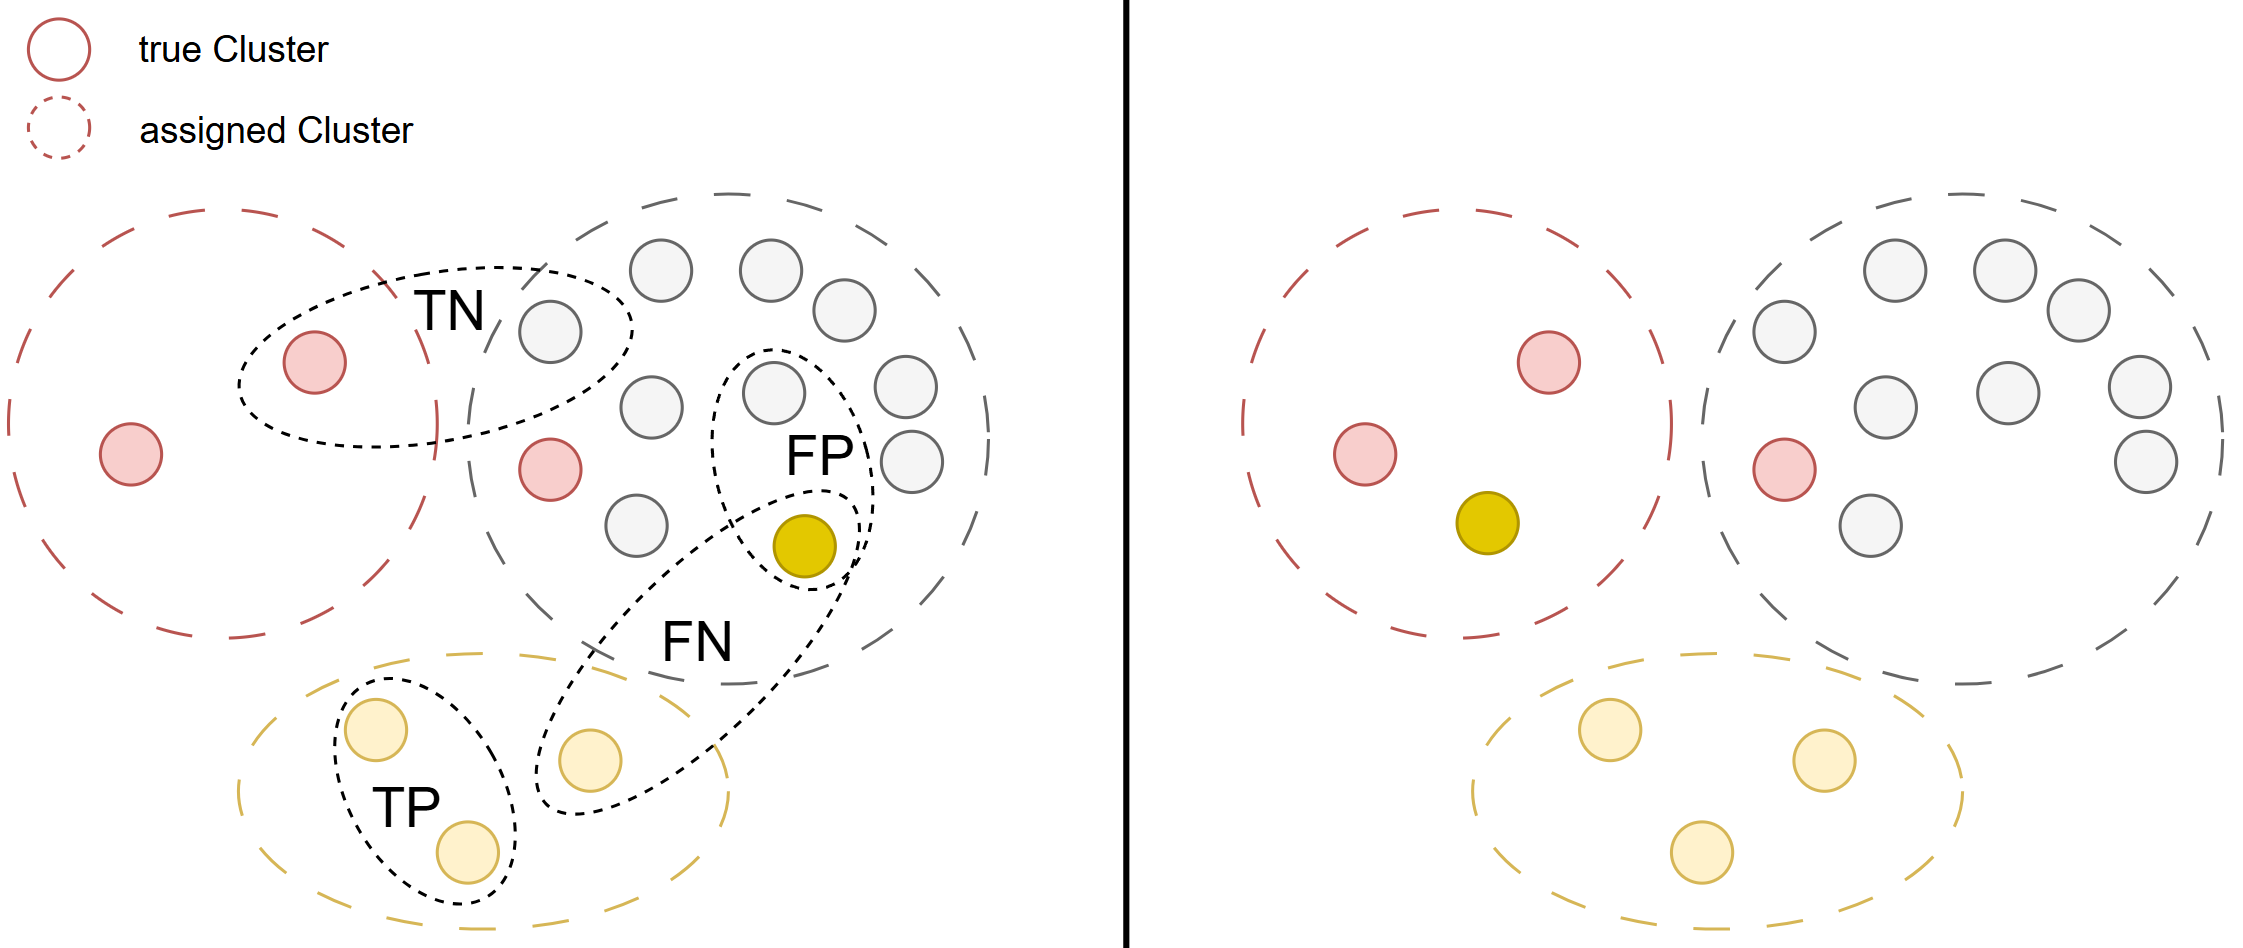
\includegraphics[width=0.9\linewidth]{plots/classes.png}
\caption{\label{fig:classes}Even though $C_{11}=41$ in both scenarios and only one item was moved between them, $C_{01} = 19$ on the left and $C_{01} = 11$ on the right side, which results in a precision metric of 0.68 on the left vs. 0.79 on the right. }
\end{figure}

To resolve this problem and avoid distortion of the confusion matrix by the noise picks, correctly classified noise was excluded from the performance calculation and each true pick which was falsely classified as noise was assigned its own cluster. 

With this approach in handling noise, true picks, which were classified as noise, are false negatives towards picks from their true clusters and therefore correctly lowering the recall, and true negatives towards all other picks, therefore not influencing precision. Noise picks, which were misclassified as real picks, count as false positives towards the cluster they were assigned to, correctly lowering precision. 

\section{GaMMA}
\subsection{Method}
We define $y := \{(\tilde{t}_j, \tilde{a}_j)^T\}^J_{j=1}$ as the set of observed picks with arrival time and amplitude, $q := \{(x_k, y_k, z_k, t_k)^T\}^K_{k=1}$ the set of earthquakes with coordinates $x_k$, $y_k$, $z_k$ and origin time $t_k$, $M := \{M_k\}^K_{k=1}$ the magnitudes and $S := \{(x_i, y_i, z_i)^T\}^I_{i=1}$ the stations.

If we have a single known earthquake $q_k$ and a measured pick arrival time $\tilde{t}_j$ at station $i$, and using the theoretical arrival time $t_{ik}$ at station $i$ of a wave produced by $q_k$, we can express our latent variable as:

\begin{equation}
    \tilde{t}_j = t_{ik} + \varepsilon 
\end{equation}

Assuming that the error $\varepsilon$ is normally distributed, and using the uniform velocity model from equation \ref{vel} with the value of $v$ depending on the phase type of $y_j$ we have:

\begin{equation}
\varepsilon = \tilde{t}_j - (t_k + \frac{d_{ik}}{v}) \qquad \varepsilon \sim \mathcal{N}(0, \sigma^2)\
\end{equation}

and therefore we can express the likelihood of pick $t_j$ belonging to event $q_k$ as:

\begin{equation}
p(\tilde{t}_j \mid q_k) = \frac{1}{\sqrt{2\pi\sigma^2}} \exp\left( -\frac{(\tilde{t}_j - (t_k + \frac{d_{ik}}{v}))^2}{2\sigma^2} \right)
\end{equation}

The same logic applies to the amplitude estimation and allows to formulate the joint density $p(\tilde{t}_j, \tilde{a}_j \mid q_k, M_k)$ as the probability of pick $y_j$ belonging to the event $q_k$. It is then possible to write the joint likelihood of the set of observations given the set of events:

\begin{equation}\label{eq:joint}
    p(y \mid \phi, q, M) = \prod_{j=1}^J p(\tilde{t_j}, \tilde{a_j}\mid \phi, q, M)
\end{equation}

with $\phi := \{\phi_i\}^K_{k=1}$ being the mixture components, i.e. $\phi_k$ is the probability of any phase pick belonging to event $q_k$. The log likelihood can then be written as:

\begin{equation}\label{eq:likelihood}
    log\,p(y \mid \phi, q, M) = \sum^J_{j=1}log\left[\sum^K_{k=1} \phi_k p(\tilde{t_j}, \tilde{a_j}\mid q_k, M_k) \right]
\end{equation}
Maximizing this expression would yield an optimal clustering to a set of earthquake parameters $q$. Expression \ref{eq:likelihood} is however difficult to solve directly and
GaMMA therefore uses the expectation maximization algorithm (EM) \citep{dempster} to address this optimization problem. Initially, using either an informed or random approach, $K$ earthquakes with magnitudes $M$ are positioned within the search area. The algorithm then alternates between the E and M steps. During the E-step, the responsibility $\gamma_{jk}$ is calculated for each phase pick $y_j$ given events $q_k$.

\begin{equation}
\gamma_{jk} = \frac{\phi_k\,p(\tilde{t}_j, \tilde{a}_j \mid q_k, M_k)}{\sum^K_{k=1}\phi_k\,p(\tilde{t}_j, \tilde{a}_j \mid q_k, M_k)}
\end{equation}

In the M-step, the mixture components as well as the hypocentres and magnitudes are updated:
\begin{align}
    \phi_k &= \frac{\sum^J_{j=1} \gamma_{jk}}{J} \\
    q_k &= \arg\min_{x_k} \sum^J_{j=1} \gamma_{jk}\,\mathcal{L}(\tilde{t}_j, t_{ik}) \\
    M_k &= \frac{1}{\sum^J_{j=1} \gamma_{jk}} \quad \sum^J_{j=1}\gamma_{jk}\,\mathcal{F}(q_k, \tilde{a}_j)
\end{align}

With $\mathcal{L}$ being a loss function between the picked arrival time and the theoretical arrival time and $\mathcal{F}$ the function to calculate the magnitude of an earthquake from its location and the measured amplitude.

GaMMA assumes a normal distribution for the error term, which means that we can reformulate Eq.\,\ref{eq:joint} as:

\begin{equation}
    p(y \mid \phi, \mu, \Lambda^{-1}) = \prod_{j=1}^J \mathcal{N}( \tilde{t_j}, \tilde{a_j}\mid \phi, \mu, \Lambda^{-1})
\end{equation}

with $\mu$ being the theoretical phase arrival times and amplitudes, and $\Lambda^{-1}$ is the covariance matrix. An initial value for the covariance needs to be chosen for the first iteration, this term is then updated after the first M-Step by comparing the updated theoretical amplitudes and arrival times with the measured ones. With these calculations, it is possible to keep iterating until the algorithm converges.

The step that has been omitted up until now, is the choice of the number of earthquakes, which is one of the most difficult parts about phase association. This problem is elegantly solved by the implementation of 3 conjugate priors. A Dirichlet Prior is being used for the mixture component $p(\phi) = \mathcal{D}(\alpha_0)$ \citep{dirichlet}, a Gaussian prior for the mean conditioned on the precision $p(\mu_k \mid \Lambda_k) = \mathcal{N}(m_0, \beta_0, \lambda_k)$ and a Wishart prior for the precision $p(\Lambda_k) = W(W_0, \nu_0)$. This procedure is detailed in \citet{bishop} and GaMMA is using the implementation from \citet{scikit-learn}.

The practical effect of these priors is that the weights of the earthquakes will be regulated automatically, and events which don't help to explain the data will be have mixture components close to zero. Therefore, the user can set the parameter K to a number larger than the expected number of events, and expect the model to decide on the number of events on its own.

The phase type information for each pick is utilized exclusively within the velocity model to select the appropriate wave velocity. Consequently, the model theoretically permits the assignment of multiple picks of the same type from the same station to a single event. It does also not account for the differences in arrival times of various wave types at a station.

Before association, the pick data is pre-processed and segmented into short pick sequences using DBSCAN \citep{dbscan} based on arrival times. This improves association performance and allows segments to be associated in parallel.

\subsection{Adaptations and Configuration}

The default GMPE implemented in GaMMA was found to be undefined for earthquakes below magnitude -2 and for distances less than 100 meters. Consequently, we implemented the relation by \citet{butler1993apquant} from Eq.\,\ref{eq:gmpe}.

Various configuration parameters can be specified to control the association. Calibrating those parameters required extensive testing and a good understanding of the underlying method, as they had to be set to values outside of their normal ranges. 

Since our dataset consists of very small amplitudes and travel times, the before mentioned initial assumption of the covariance prior $\Lambda^{-1}$ for time and amplitude is crucial. Values of 1e-5 for time and 1e-2 for amplitude achieved significantly better results than the dynamic choices by the algorithm. Similarly, the DBSCAN \textit{eps} parameter, controlling the maximum distance between two samples for one to be considered as in the neighborhood of the other, was reduced from 10s to 0.01s to account for the small time scale. Those configurations had the largest impact in allowing GaMMA to work in this specific use-case.

It is possible to filter out clusters below certain thresholds. A maximum sigma for time and amplitude can be chosen independently. Those values will depend mostly on the seismic network and its quality of the data, in case of larger uncertainties and more noise picks, a larger value will have to be selected. For the synthetic test data, a maximum $\sigma_t$ of 0.01 and a maximum $\sigma_a$ of 2 were chosen. It is possible to select the minimum number of required picks per cluster in a similar way. Depending on the density of the monitoring station, this value should also be adjusted accordingly, since in a denser network, an earthquake should be detected by more stations. Tests showed that a minimum of 8 stations provided good results in the tests data.

Given that GaMMA routinely segments longer pick sequences into shorter ones, most tests and performance evaluations were conducted on sequences ranging from 0.1s to 300s. This approach not only speeds up association but also simplifies data management.

\chapter{Results}
Initially, the overall performance of GaMMA and PyOcto was evaluated using a series of short datasets (Fig. \ref{fig:performance}). For a set of event rates from 1 to 51 events per second, 50 random catalogues, each lasting 60 seconds were generated using the previously described methodology.

As anticipated, both methods demonstrated robust performance at relatively low earthquake rates. Their effectiveness remained comparable at a rate of one event per second. However, PyOcto's performance began to decline rapidly as the event rate increased.

\begin{figure}[ht]
    \centering
    \begin{minipage}{0.42\textwidth}
        \centering
        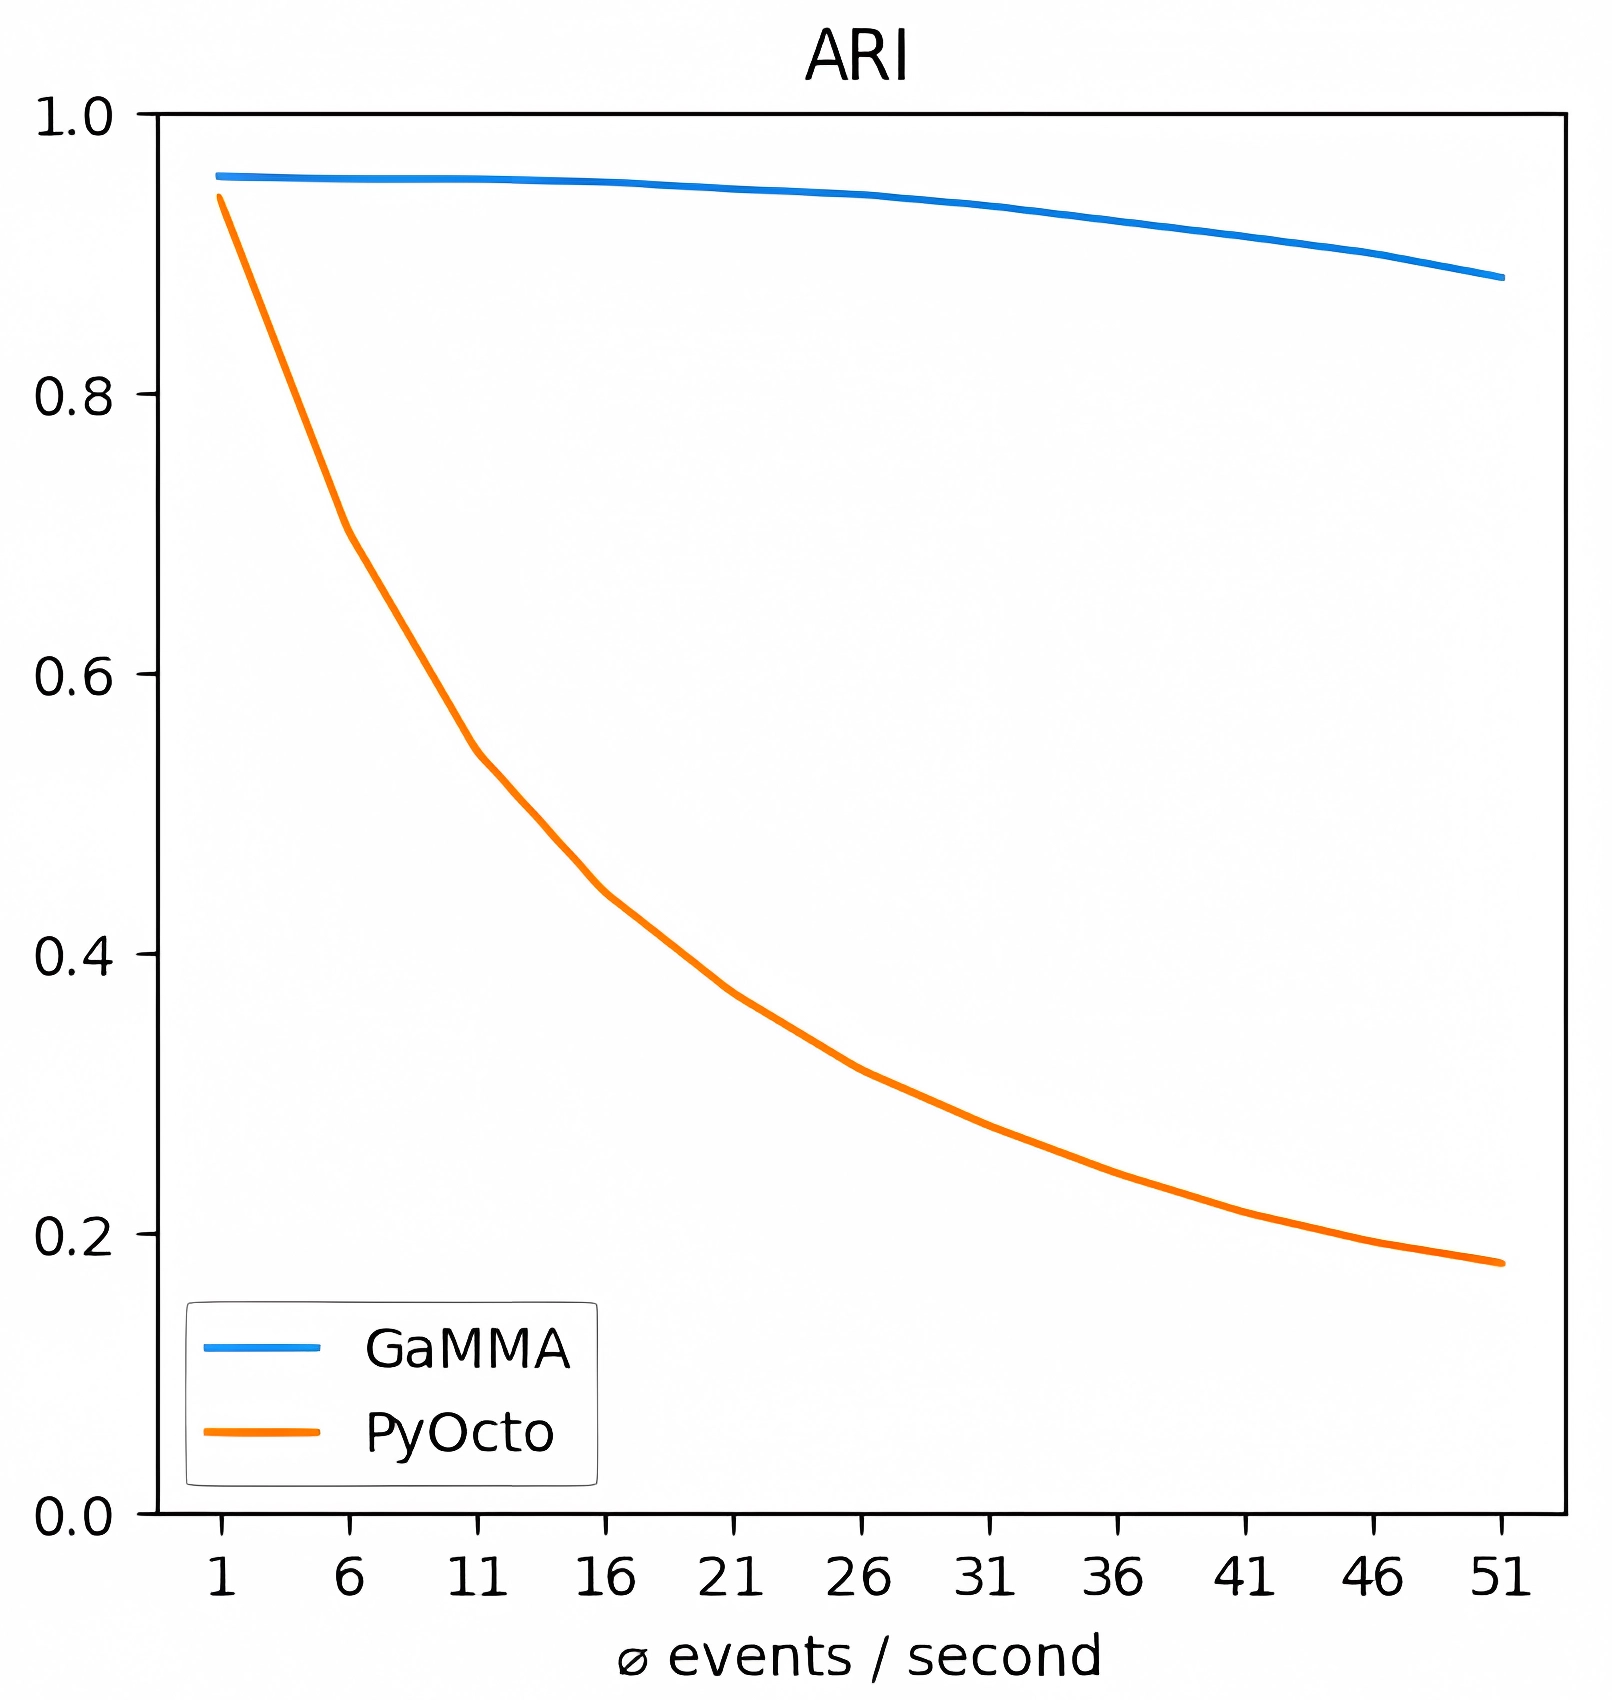
\includegraphics[width=\textwidth]{plots/performance_comparison_ari.png}
    \end{minipage}
    \hfill
    \begin{minipage}{0.42\textwidth}
        \centering
        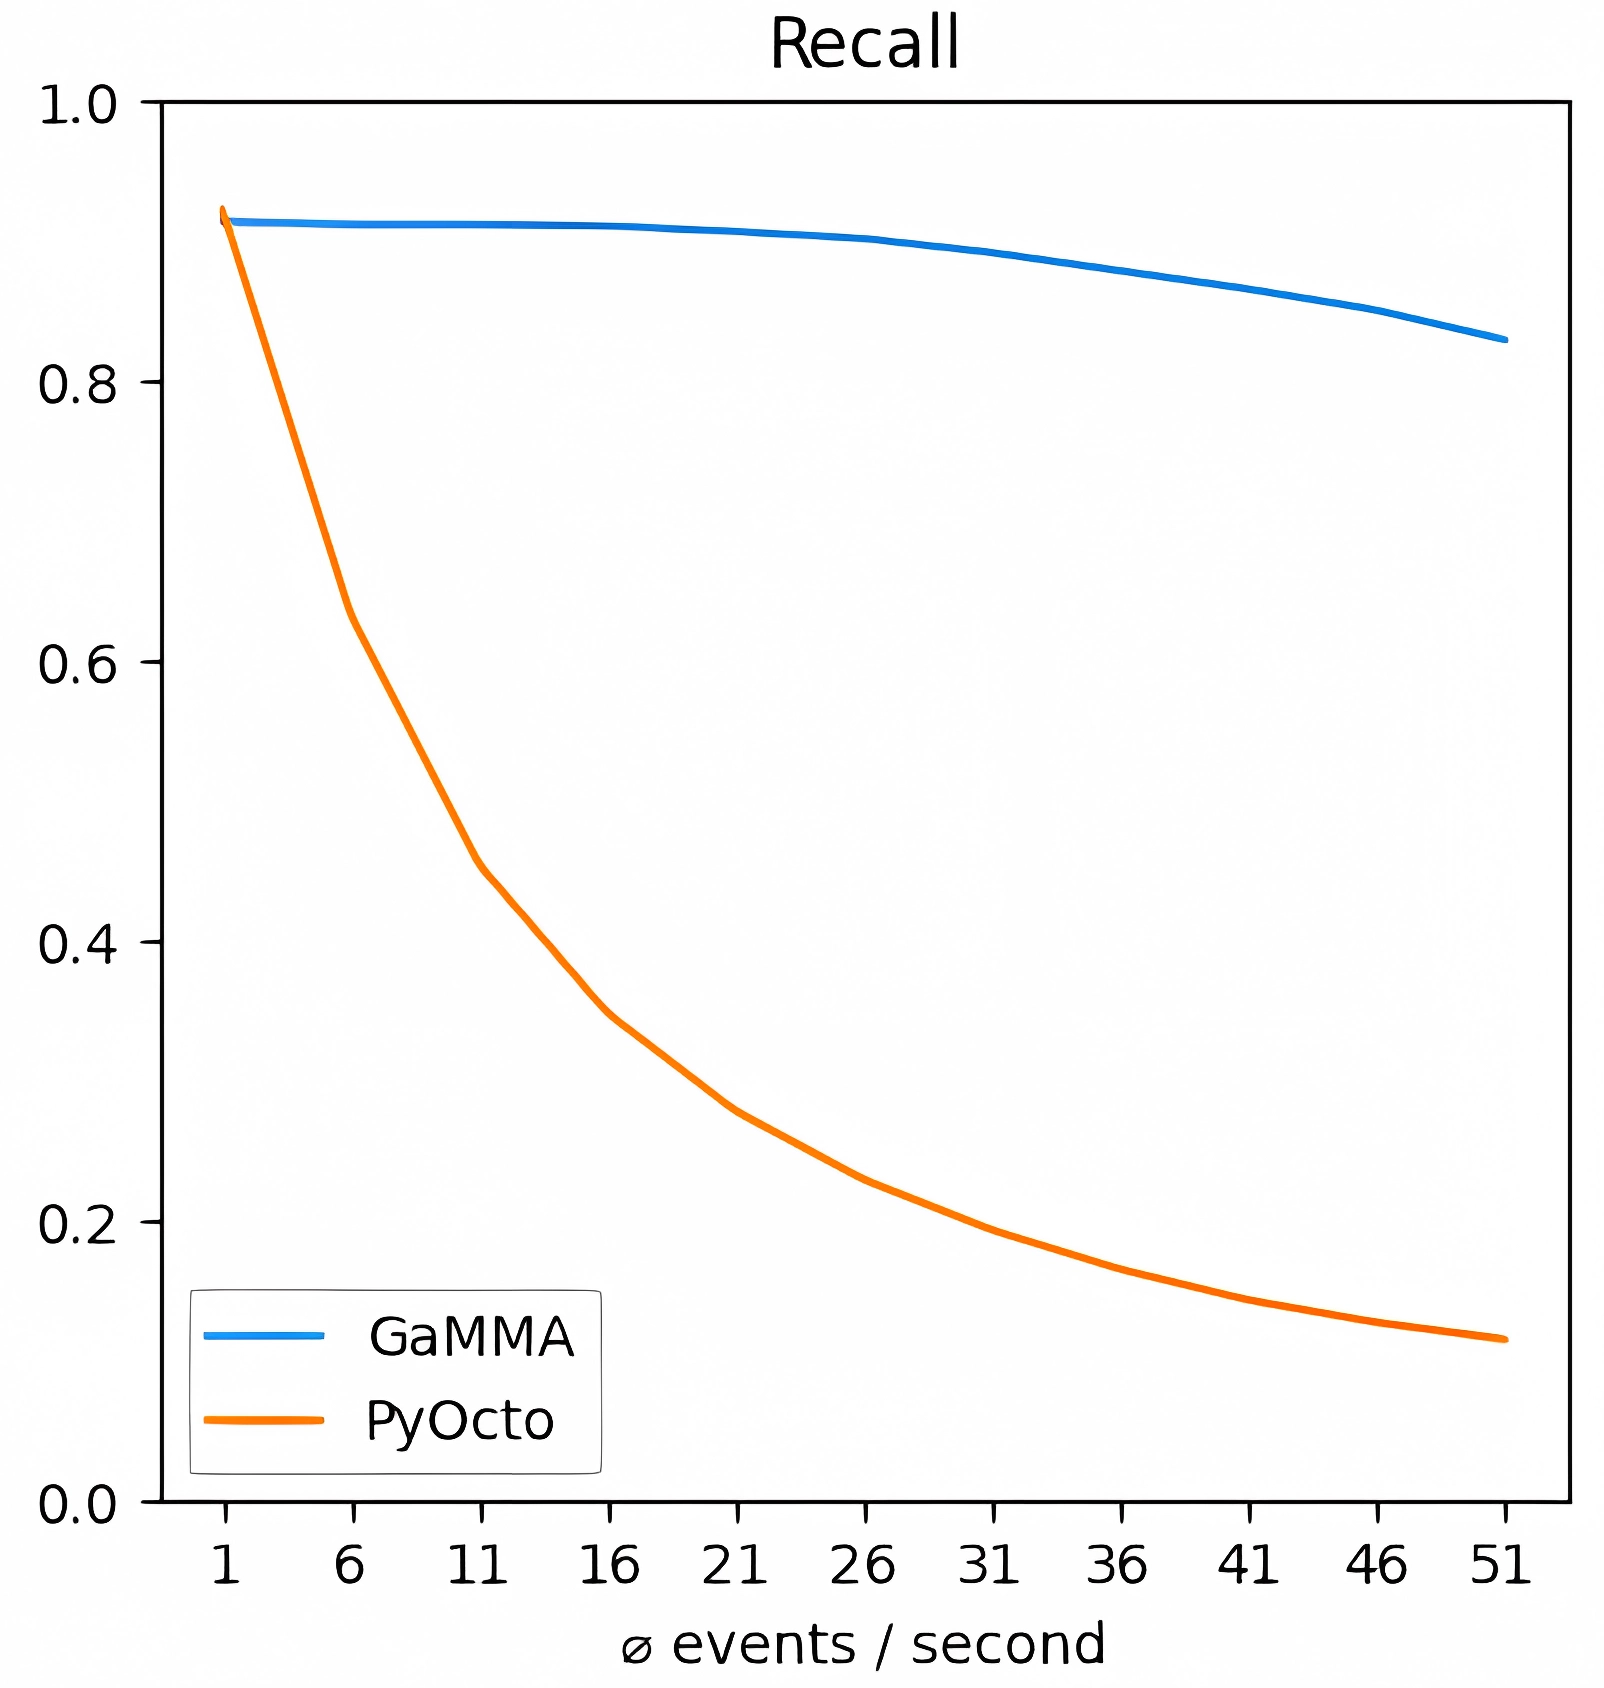
\includegraphics[width=\textwidth]{plots/performance_comparison_recall.png}
    \end{minipage}
    \caption{\label{fig:performance}Comparison of adjusted rand index and recall for GaMMA and PyOcto for increasing number of events per second.}
\end{figure}

Creating synthetic data by sampling event times using a Poisson Process makes it challenging to precisely quantify the event rate at which the method fails. To address this, a dataset was constructed with events evenly spaced in time, while magnitudes and locations were randomly sampled using the previously described methodologies. This approach allows for a more detailed observation of when and how the method begins to miss a significant share of the events.

If we only consider the arrival time information, then the performance starts to drop off above a rate of 40 events per second (Fig.\,\ref{fig:perf_fix_time}). At that rate, the time between events is about the same as the S-wave travel time from the events to the farthest recording station. Therefore recordings of picks from multiple events will start to overlap and association becomes significantly more difficult, as expected. If we also use the amplitude information (Fig.\,\ref{fig:perf_fix_phase}), then the method starts out with a lower performance, but is more robust once the events start overlapping.

\begin{figure}[h]
    \centering
    \begin{minipage}{0.47\textwidth}
        \centering
        \caption{\label{fig:perf_fix_time}Events with evenly spaced origin times}
        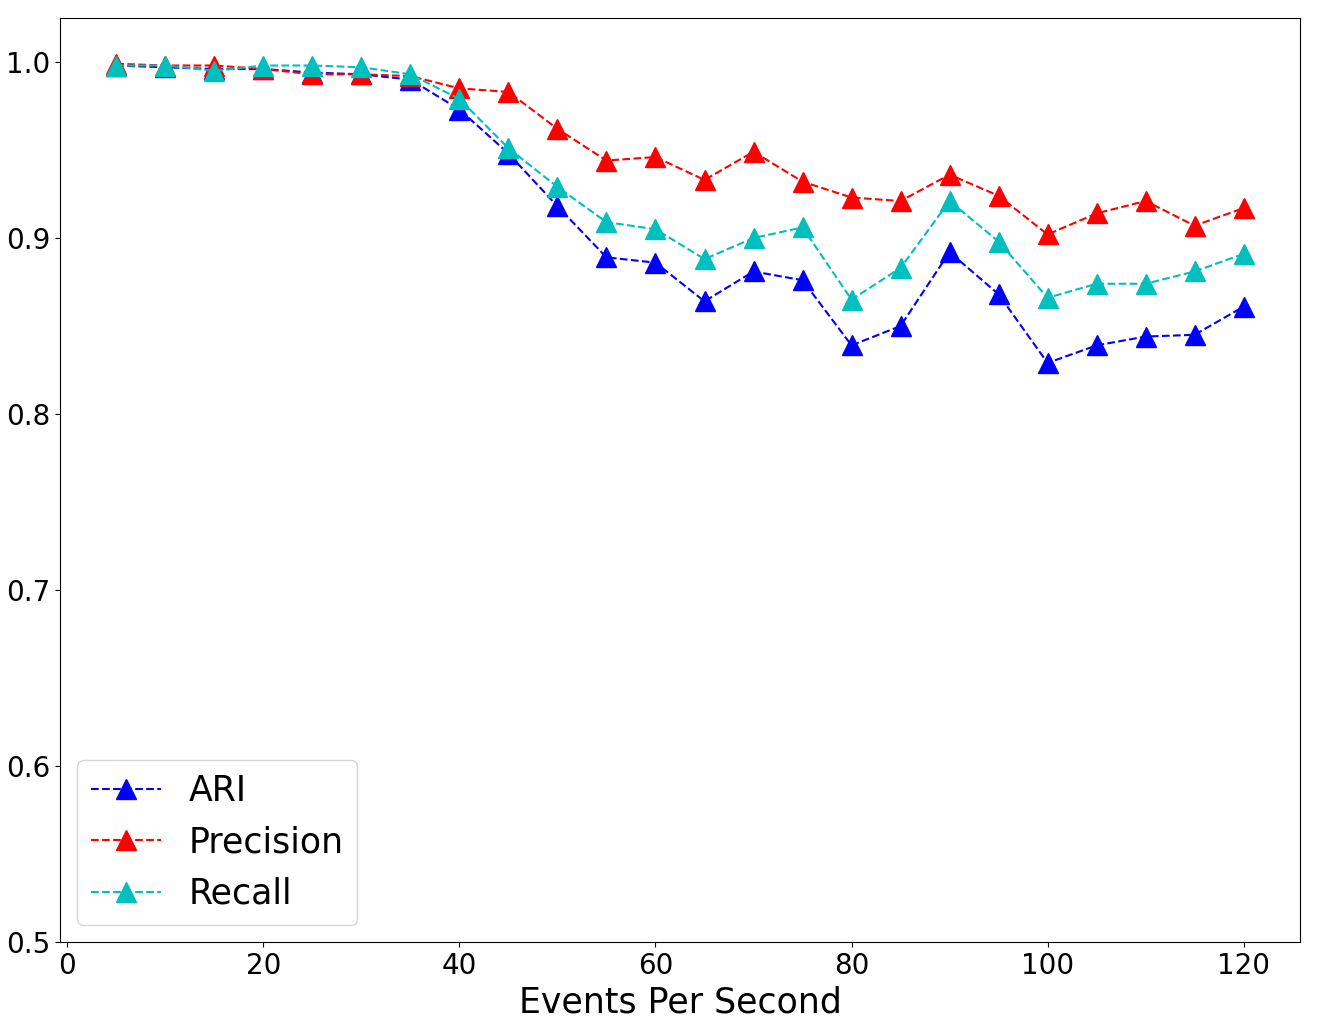
\includegraphics[width=\textwidth]{plots/performance_gamma_fix_time.png}
    \end{minipage}
    \hfill
    \begin{minipage}{0.47\textwidth}
        \centering
        \caption{\label{fig:perf_fix_phase}Events with evenly spaced origin times, with amplitude}
        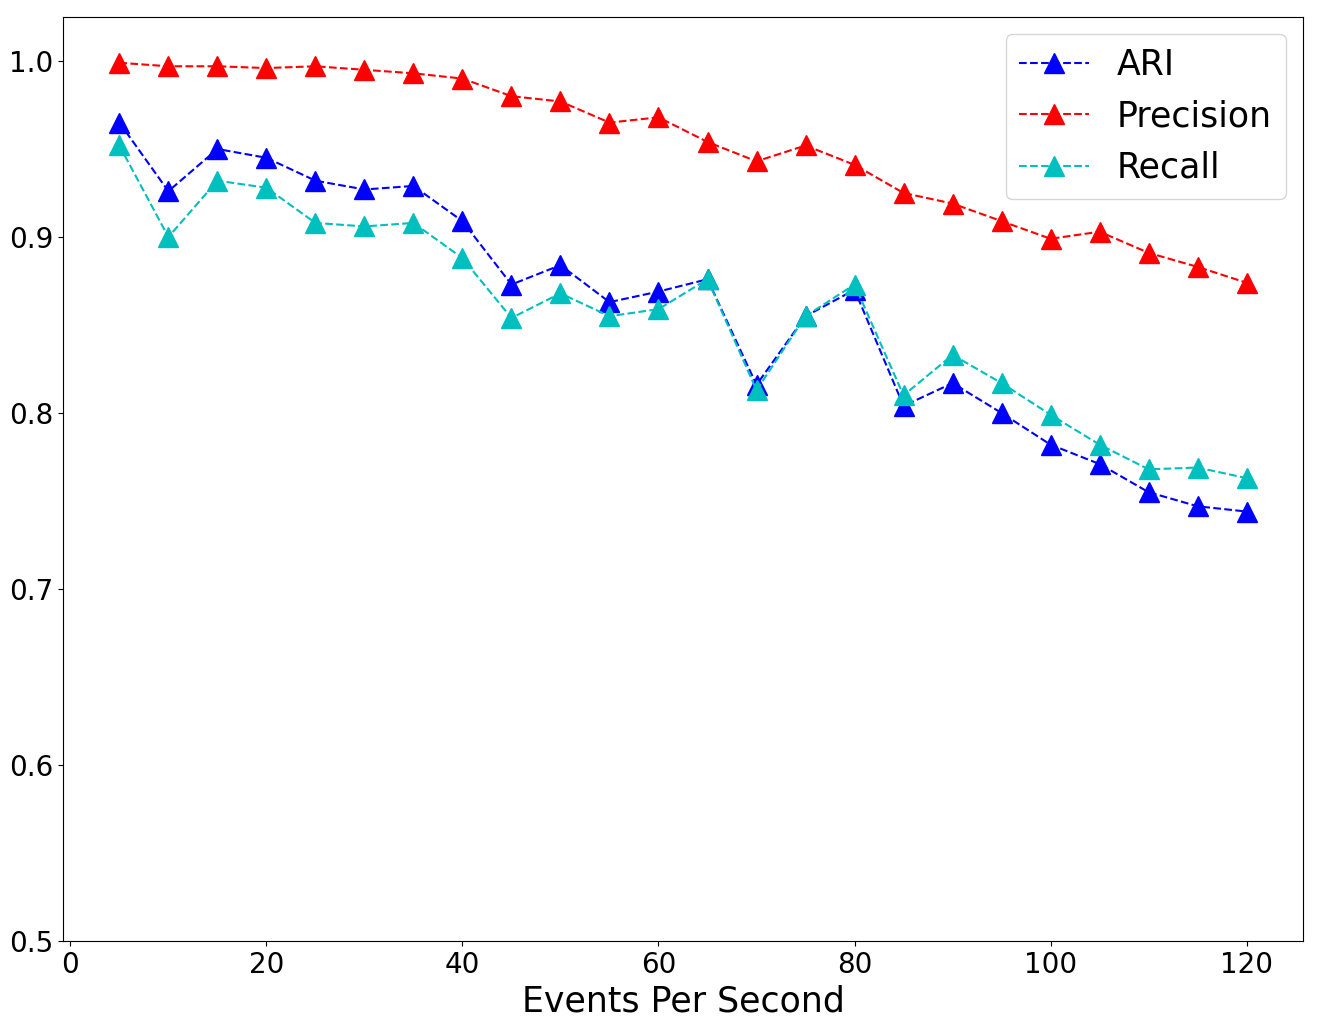
\includegraphics[width=\textwidth]{plots/performance_gamma_fix_phase.png}
    \end{minipage}
        \centering
    \begin{minipage}{0.47\textwidth}
        \centering
        \caption{\label{fig:perf_time}Events with Poissonian arrival times}
        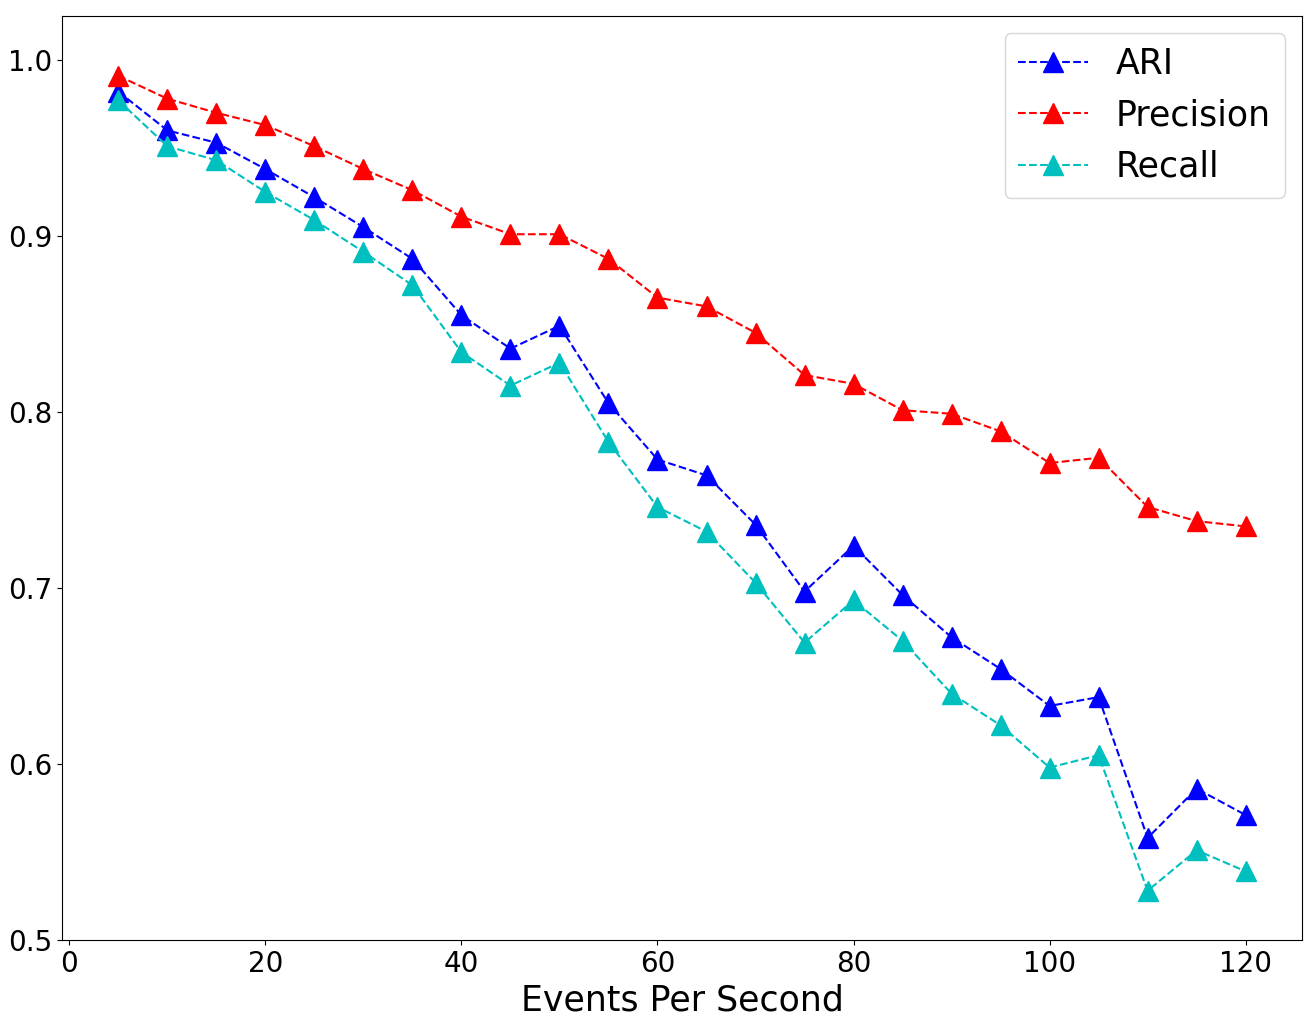
\includegraphics[width=\textwidth]{plots/performance_gamma_time.png}
    \end{minipage}
    \hfill
    \begin{minipage}{0.47\textwidth}
        \centering
        \caption{\label{fig:perf_phase}Events with Poissonian arrival times, with amplitude}
        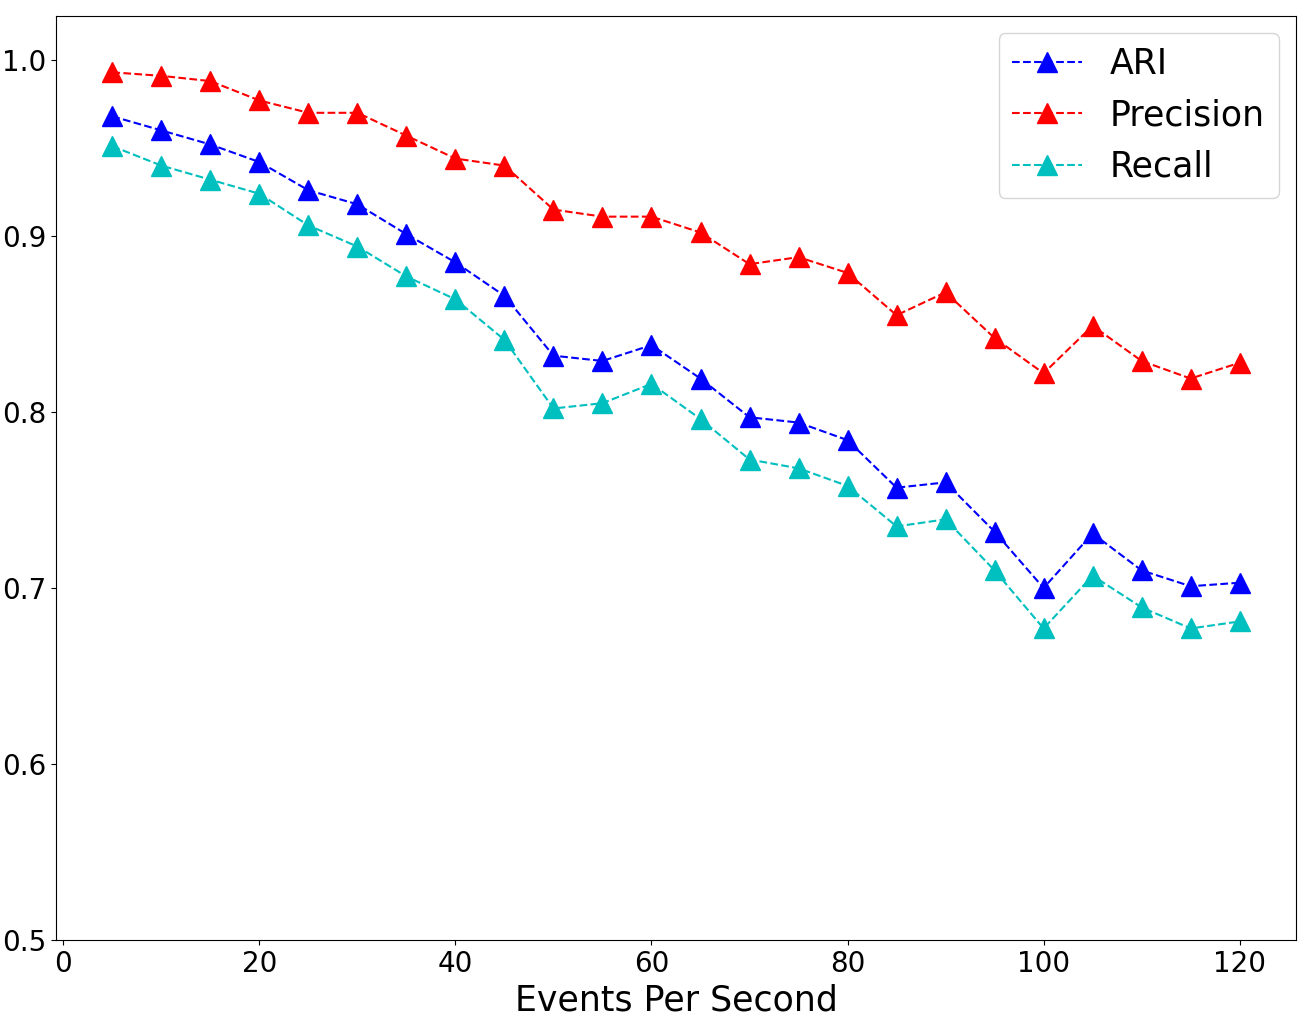
\includegraphics[width=\textwidth]{plots/performance_gamma_phase.png}
    \end{minipage}
\end{figure}

On a dataset where event times were generated using a Poisson Process (Fig.\,\ref{fig:perf_time}), performance deteriorated much more rapidly. The Poisson Process does not ensure well-separated event times, allowing for the possibility of multiple events occurring in quick succession. This represents a more realistic scenario, as earthquakes often occur in clusters. However, when amplitude information was also considered (Fig.\,\ref{fig:perf_phase}), performance remained above 0.8 for event rates of up to 60 events per second.

In Fig.\,\ref{fig:clusterings}, two challenging examples are illustrated, showcasing the some of the complexities of the problem. In the first part of the upper example, two large events 
are overlapping, complicating the association process. The subsequent red cluster is partially associated correctly, though the earthquake location is far off, leading to some picks being incorrectly associated. The lower sequence in Fig.\,\ref{fig:clusterings} displays events with origin times generated using a Poisson process. Toward the end of this sequence, a dense cluster of events occurs, presenting a scenario where GaMMA unsurprisingly struggles in accurately associating the picks.


\begin{sidewaysfigure}[h]
    \centering
    \begin{minipage}{1\textwidth}  % Adjusting width to 80% of text width
        \centering
        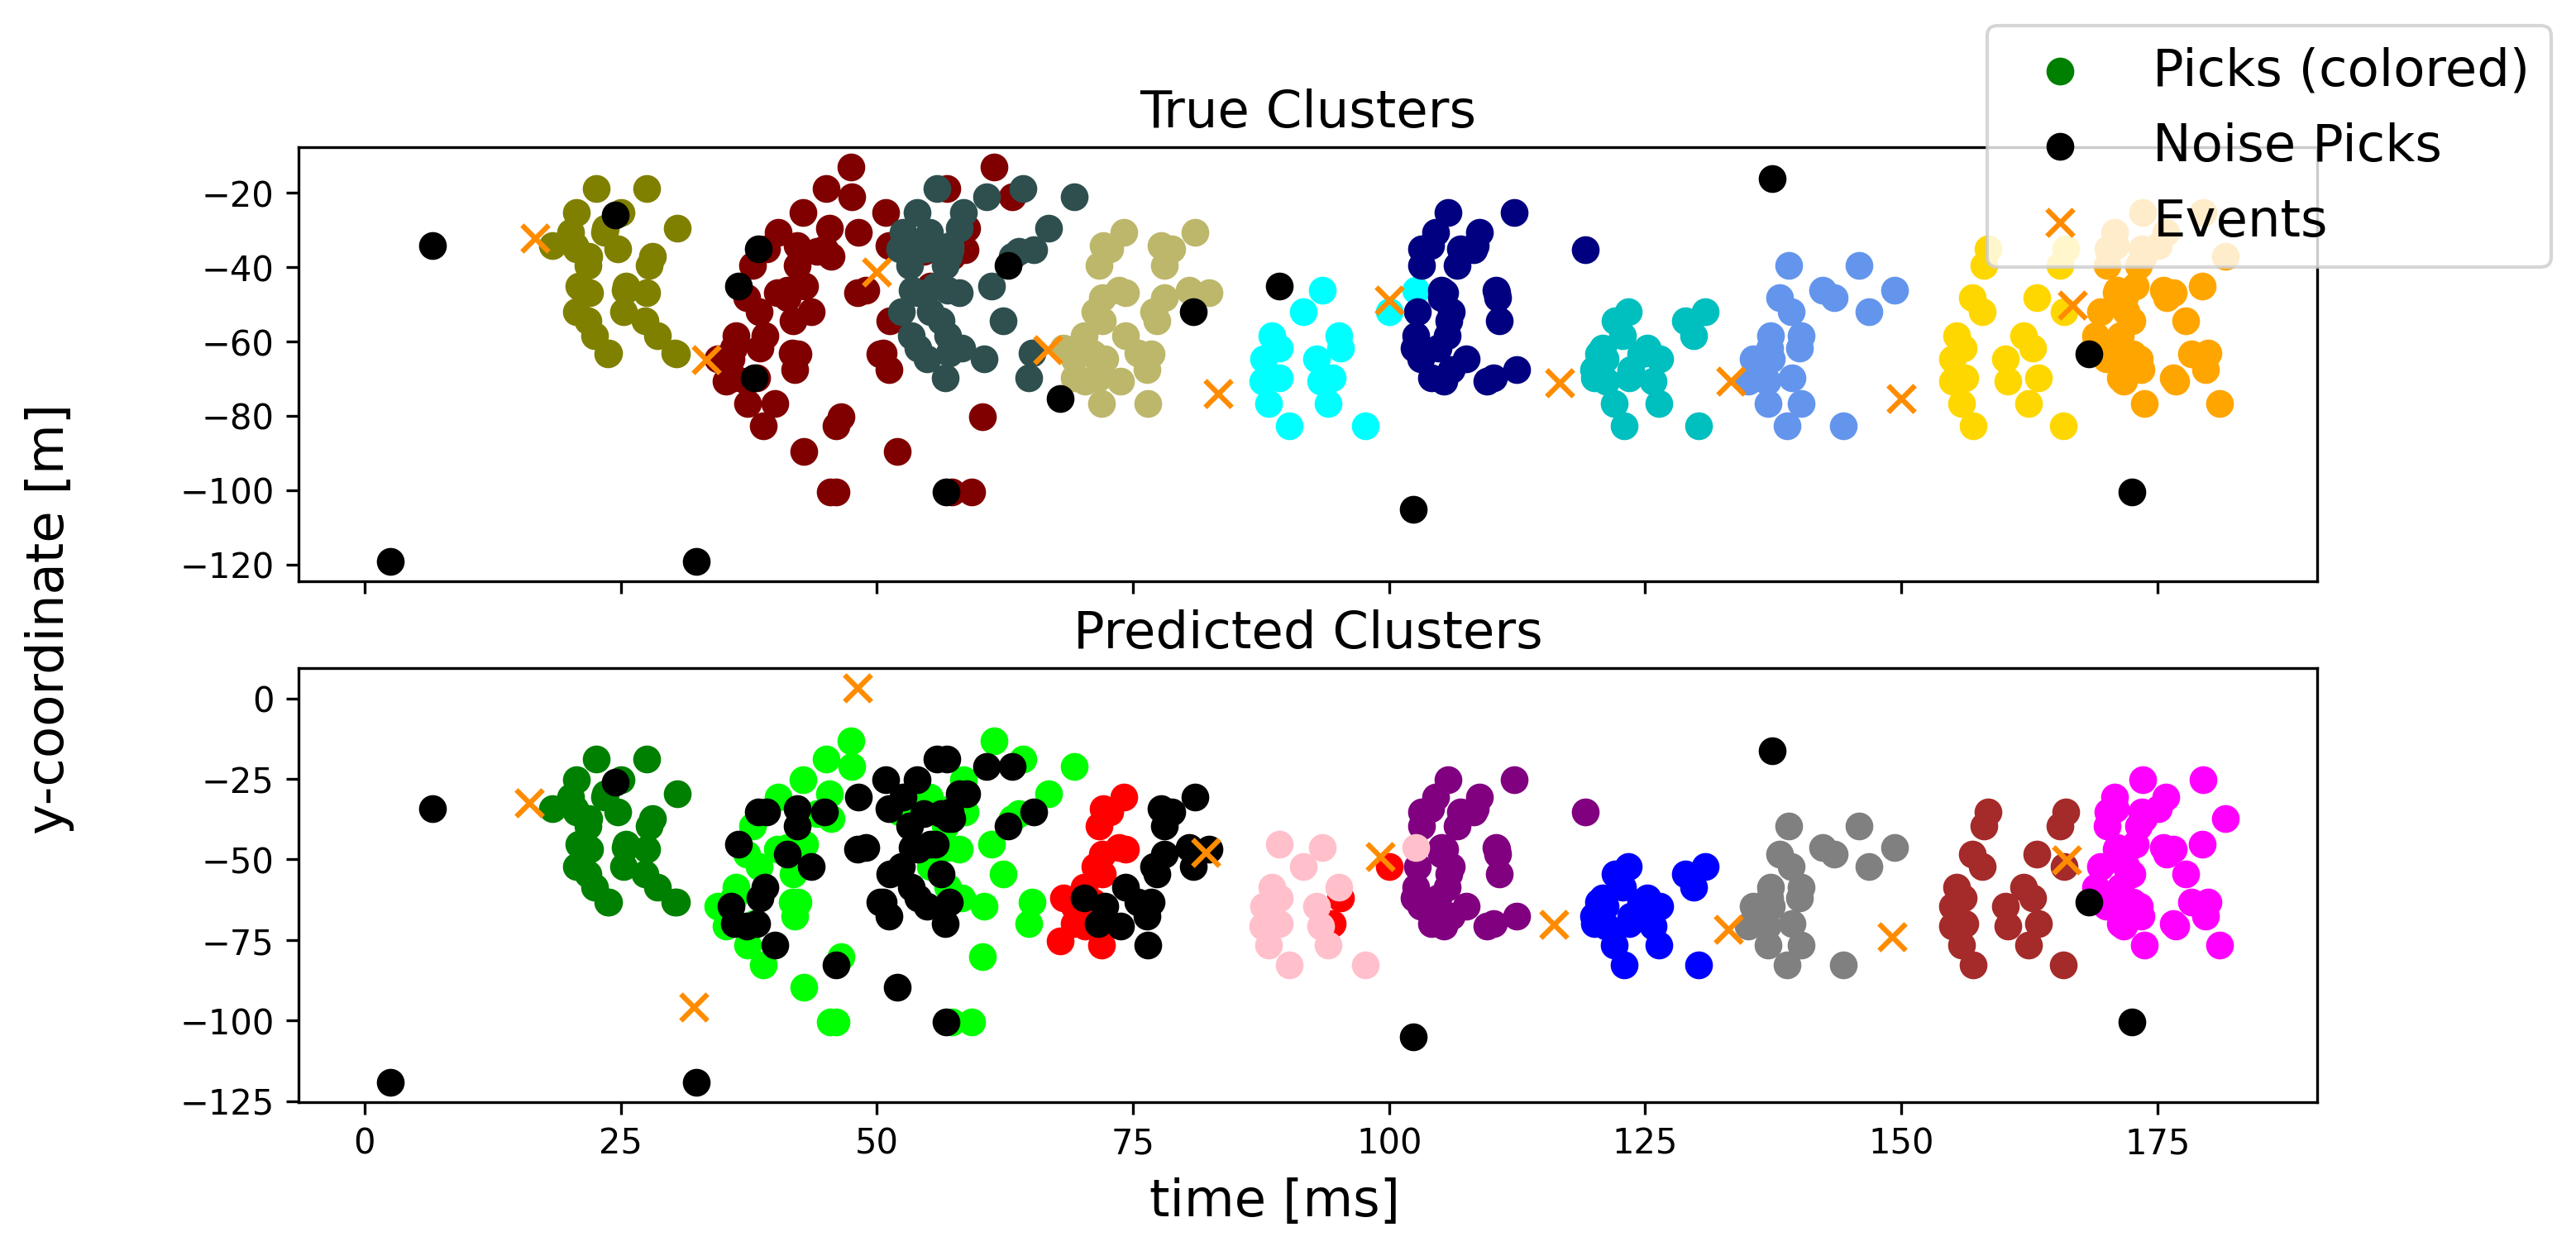
\includegraphics[width=\textwidth, height=0.35\textheight, keepaspectratio]{plots/clustering_full_regular.png}  % Set height to 40% of text height
    \end{minipage}
    \vfill
    \begin{minipage}{1\textwidth}  % Adjusting width to 80% of text width
        \centering
        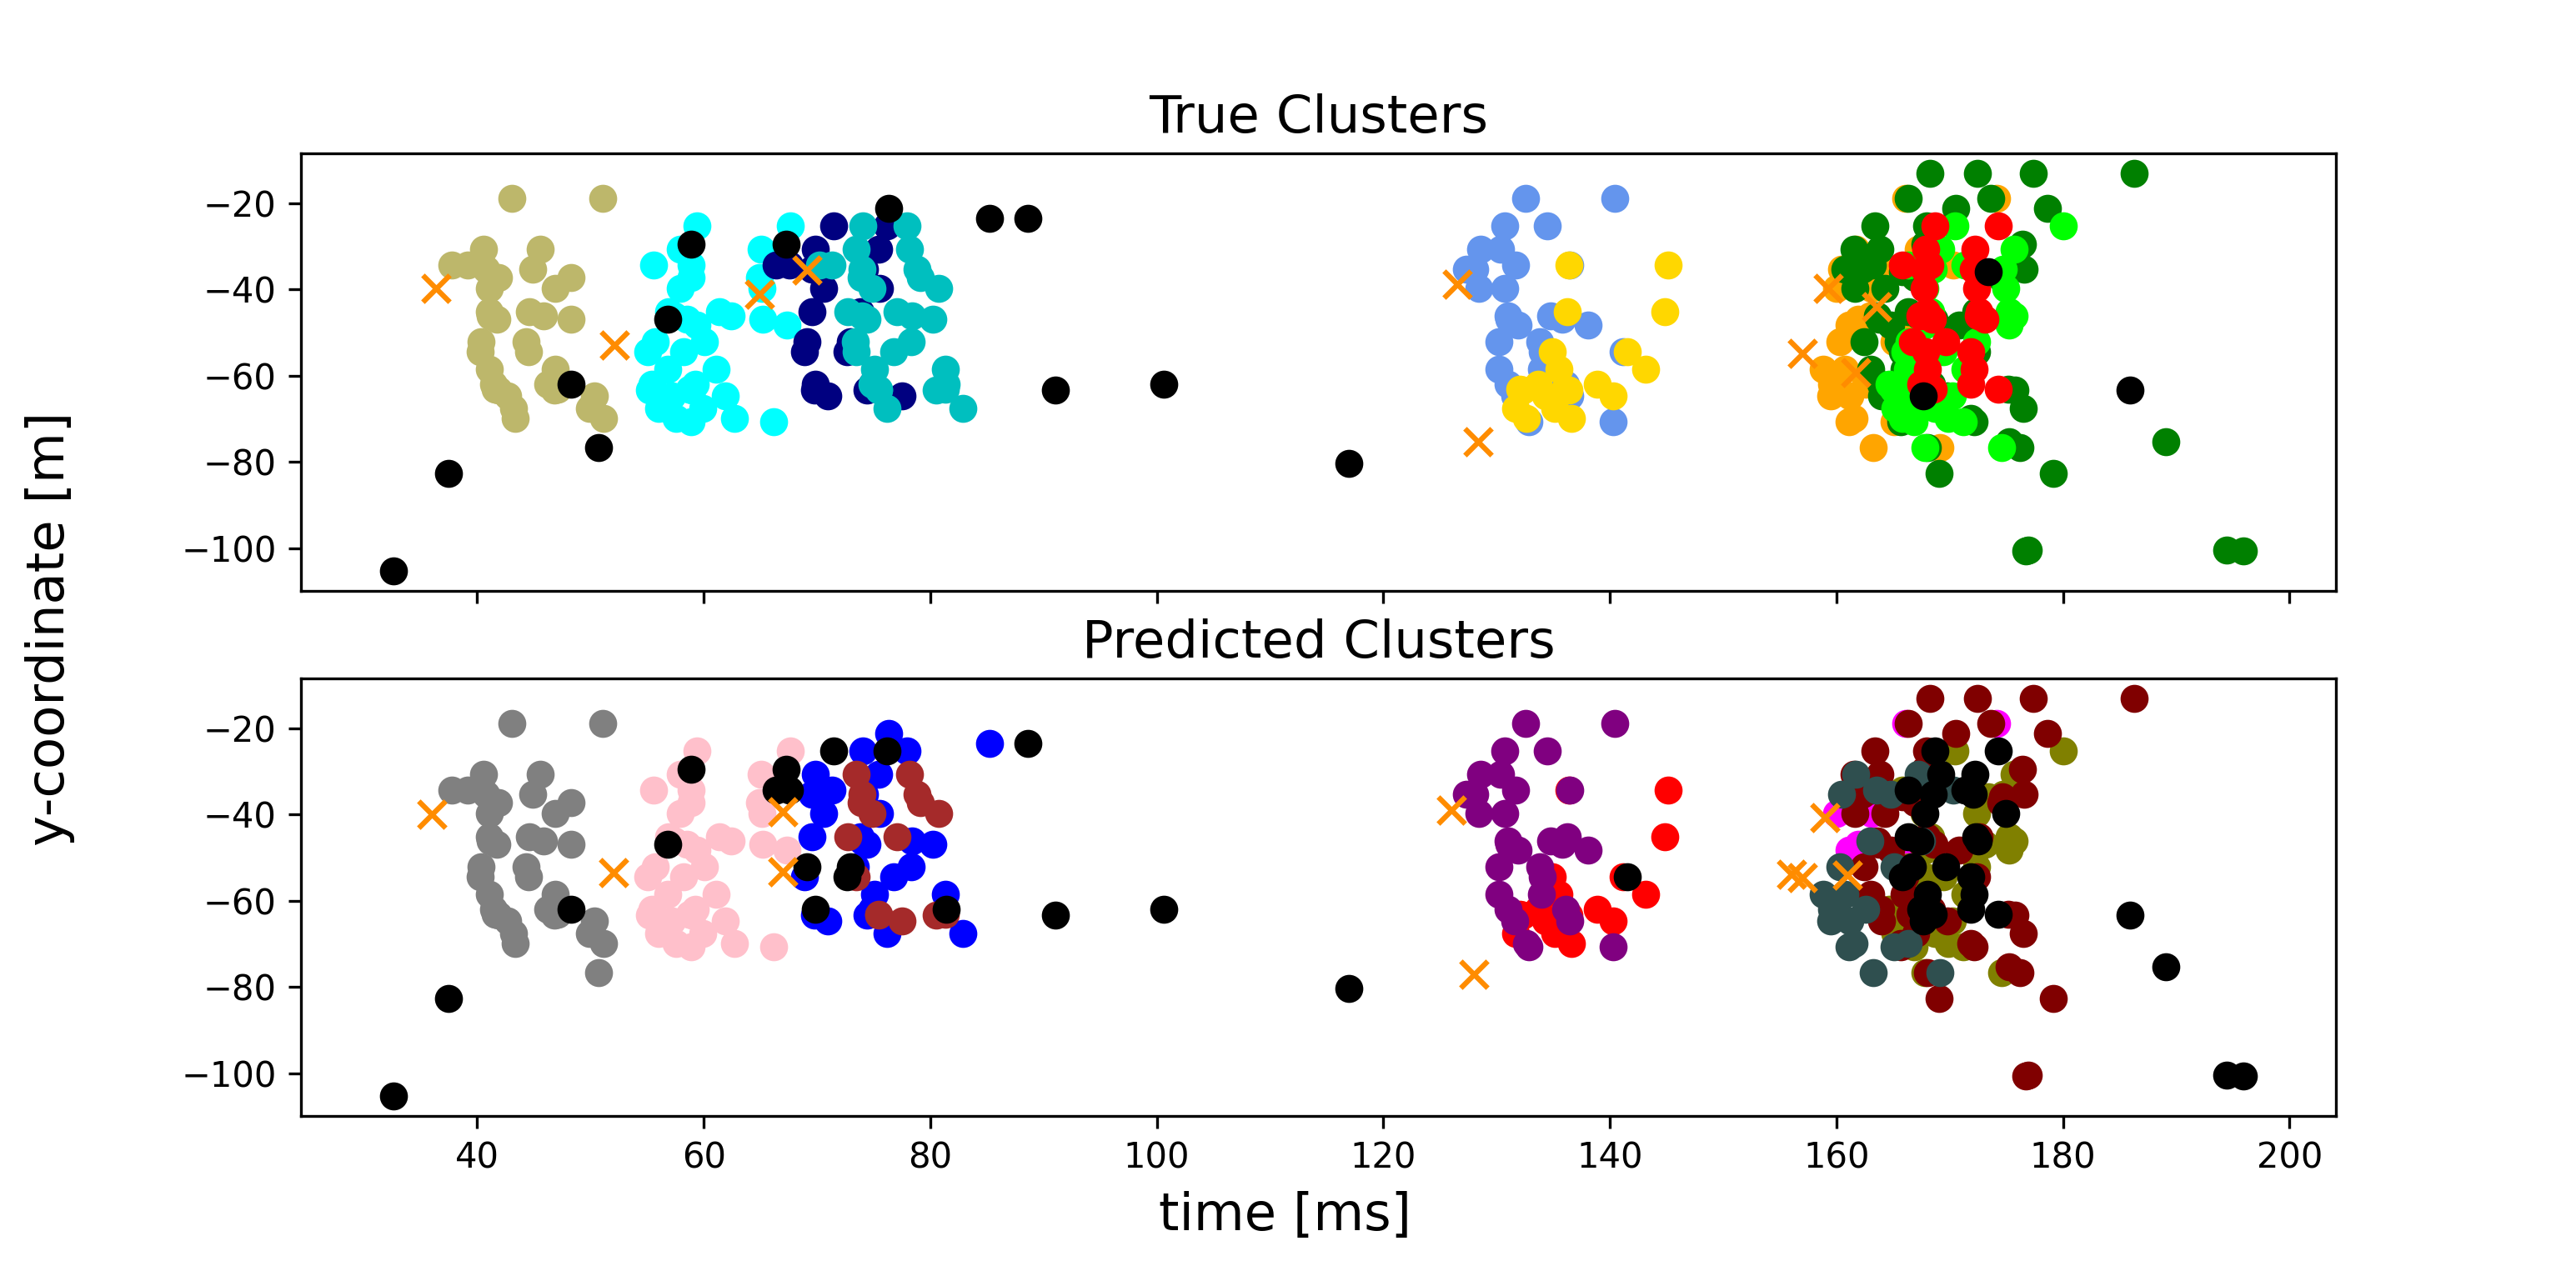
\includegraphics[width=\textwidth, height=0.352\textheight, keepaspectratio]{plots/clustering_full_irregular.png}  % Set height to 40% of text height
    \end{minipage}
    \vfill
    \parbox{0.8\textwidth}{  % Adjust the width here
    \caption{\label{fig:clusterings}Pick times vs. station y-coordinates.}
    }
\end{sidewaysfigure}


\chapter{Discussion}
While various methods for phase association could potentially be adapted to this specific context, many of the proposed algorithms appear unrealistic for practical application at BedrettoLab or a geothermal site. Furthermore, numerous methods have not been actively utilized post-development, or they require significant effort to implement and train. In contrast, both PyOcto and GaMMA offer comprehensive documentation, are open-source, and remain actively maintained and utilized.

Even with careful and thorough testing, we could not adapt PyOcto in its current implementation to the scale required by BedrettoLab. Optimization of the PyOcto implementation was beyond the scope of this work, since we deemed it less likely that classic methods like PyOcto, which use a form of grid search and back-projection, will tackle the scale needed for this use-case.

However, we could show, that with a well configured and adapted implementation of GaMMA it is possible to achieve good results in scenarios very similar to what would be expected in BedrettoLab. Additionally, a method was developed to create synthetic data for such scenarios, as well as for measuring the performance of the algorithms, which will both facilitate further improvements and implementations of an adapted phase picking algorithm for BedrettoLab.

Multiple possible areas for improvement could be identified, some of them also already mentioned in the original GaMMA paper, and others proven to be effective in a separate standalone implementation NEUMA by \citet{neuma}. One such area lies in adaptations to the overall scheme. A better initialization of the hypocentres could enhance overall performance and accuracy. By differentiating between P- and S-picks it could be possible to disallow certain assignments or improve the hypocenter location estimation. NEUMA also proposes to use Laplacian distributions for the error estimates and introduced an additional mixture component to account for the noise.

The greatest potential for improvement likely lies in refining wave travel estimation and amplitude calculation. Conceptually, they could be treated as plug-in modules, allowing for the development and integration of specialized methods, while not changing the overall approach. Also, these methods are not constrained to physical or empirical relationships, and could easily be replaced by deep learning algorithms.

Regrettably, GaMMA lacks this modularity at the moment. It has implemented its algorithm by copying relevant files from the \textit{scikit-learn} library \citep{scikit-learn} and modifying the necessary methods. Therefore, some additional effort is required to enable easy integration of such extensions as mentioned above. This would, however, enable a more flexible adaptation to diverse seismic monitoring scenarios and improvements in performance and accuracy of the method.


\printbibliography

\end{document}
